\documentclass{ucbthesis}

%%%%%%%%%%%%%%%%%%%%%%%%%%%%%%%%%%%%%%%%%%%%%%%%%%%%%%%%%%%%%%%%%%%%%
\usepackage[T1]{fontenc}         % Use T1 encoding instead of OT1
\usepackage[utf8]{inputenc}      % Use UTF8 input encoding
\usepackage{microtype}           % Improve typography
\usepackage{booktabs}            % Publication quality tables
\usepackage{amsmath}
\usepackage{amsfonts}
\usepackage{mhchem}
\usepackage{graphicx}
\usepackage{gensymb}
\usepackage{float}
\usepackage{subcaption}
% \usepackage[demo]{graphicx} % the demo option is just for the example
% \usepackage{capt-of}
\usepackage[exponent-product=\cdot]{siunitx}
\usepackage[colorlinks,breaklinks]{hyperref}
\hypersetup{linkcolor=black, citecolor=black, urlcolor=black}

\usepackage{lipsum}

\def\equationautorefname{Eq.}
\def\figureautorefname{Fig.}


%%%%%%%%%%%%%%%%%%%%%%%%%%%%%%%%%%%%%%%%%%%%%%%%%%%%%%%%%%%%%%%%%%%%%


\begin{document}

\title{An Angle-Informed Hybrid Method for CADIS and FW-CADIS}

\author{Madicken Munk}
\author{Rachel N. Slaybaugh}
\affil{Department of Nuclear Engineering \\
  University of California, Berkeley
  3115B Etcheverry Hall, Berkeley, CA \\
  madicken@berkeley.edu}

\maketitle

\chapter{Literature Review}
The following literature review aims to contextualize the work described in this
dissertation within the realm of hybrid methods for deep-penetration
neutron transport. In doing
so, it will describe pertinent theoretical information that is relevant to this
topic. This will be supplemented by a discussion of the various efforts
to use these methods practically and the degree to which those methods succeeded.
First a brief overview of variance reduction for monte carlo radiation transport
will be described in section \ref{sec:MCvar}.
This will then transition in section \ref{sec:AutomatedVR} into an elaboration
of various efforts to automate variance reduction techniques within monte carlo.
Following that, section \ref{sec:Importance} will introduce the concept of
importance and how that relates to variance reduction. This section will also
focus specifically on how the adjoint solution of the neutron transport equation
relates to importance.
From this point, the chapter will transition
from theory into existing implementations
of variance reduction techniques used in modern software in the nuclear
engineering community. This will begin in \ref{sec:CADIS} with a description of
the consistent, adjoint-driven importance sampling, or CADIS, and
forward-weighted CADIS (FW-CADIS) methods.
The following section, \ref{sec:AngleVR}, will detail the efforts to incorporate
angular information into variance reduction methods for Monte Carlo.
The sections on CADIS, FW-CADIS, and angle-specific variance reduction
techniques will be concluded with with a description of the
various software in which these methods have been implemented and the degree to
which they have been successful.

\section{Monte Carlo Variance Reduction}
\label{sec:MCvar}

Monte Carlo methods for radiation transport are used in the nuclear
engineering community for a wide spectrum of application problems. Without any
variance reduction techniques, Monte Carlo methods aim to emulate
the transport of a particle from birth, through physical interaction, to death
by randomly sampling probabilities particle production, elastic and inelastic
scattering, and absorption for that particle.
This process of transporting a single particle
is repeated millions of times, which is analogous to transporting
millions of particles throughout the problem. When the user achieves a
sufficient
number of particles to sample to reach the desired statistical precision for
the region of interest, the
simulation will be complete. However, this naive approach to simulating each
particle, no matter whether it is likely to contribute to the tallied result,
can be extraordinarily computationally inefficient depending on the problem. A
user could waste time simulating millions of unusable particles and still not
reach the desired statistical precision for the tally. Variance
reduction techniques were developed to address this issue. In general, these
techniques bias the Monte Carlo transport to more effectively
contribute to a particular result, while not fundamentally changing the nature
of the problem being solved.

\subsection{Statistical Background}
\label{subsec:StatBkgnd}

Variance reduction techniques are rooted in statistics, so we will begin our
discussion of variance reduction techniques with a brief primer on the
statistical background relevant to Monte Carlo radiation transport. Sections
\ref{subsubsec:PopStat} through \ref{subsubsec:FOM} are summarized from
\cite{lewis_computational_1984} and \cite{mcnp_manual_v1}.
Monte Carlo
methods transport many randomly sampled
particles, and when those particles reach a region of interest, they are scored
in a tally. The statistical precision of the tally
will reflect the total number of particles that were sampled in- or at- this
region or surface.
The reliability of the answer obtained in this region is then dependent
on the quantity of these particles,
and the amount of time taken to move the particles on
their respective random walks through space to the region.

\subsubsection{Population Statistics}
\label{subsubsec:PopStat}

In radiation transport, one desires to estimate some response in phase-space.
This response is the average behavior of the physical interactions in some
differential phase-space in energy, space, or time. If the probability density
function $f(x)$ for the response is known exactly,
then the response in $dx$ can be calculated exactly by the true
mean, or
\begin{equation}
  \bar{x} = \int_{-\infty}^{\infty} xf(x) dx .
\end{equation}
Rarely $f(x)$ is known
exactly, so instead it is sampled.
Using $N$ randomly sampled particles, the estimate of the true mean value is given as
\begin{equation}
  \hat{x} = \frac{\sum_{i=1}^{N}{x_i}}{N} ,
\end{equation}
where $x_i$ is the i$^{th}$ event. $\hat{x}$ is the sample mean, or the
estimated value of $\bar{x}$
based on the $N$ number of samples that were used to calculate $\hat{x}$. As $N
\rightarrow \infty$, $\hat{x}$ will $\rightarrow \bar{x}$, which is given by the
Strong Law of Large Numbers \cite{mcnp_manual_v1}.
$\hat{x}$ in itself is a useful measure, but determining the spread of values
about $\hat{x}$ is also an important measure. This is called the variance. The
true variance of the distribution is
\begin{equation}
  \sigma^{2}\big( x \big) = \bar{x^2} - \bar{x}^2 ,
\end{equation}
and the standard deviation is the square root of the variance
\begin{equation}
  \sigma\big(x \big) = \big( \bar{x^2} - \bar{x}^2 \big)^{1/2}.
\end{equation}
The variance of the sampled distribution differs, as a finite number of samples
are used to calculate $\bar{x}$ and $\sigma$. The sample variance is defined by:
\begin{equation}
S^{ 2 }=\sum _{ i=1 }^{ N }{ \frac { (x_{ i }-\hat { x } )^{ 2 } }{ N-1 }  }
             \cong \widehat{x^2}-\hat{x}^2 ,
\label{eq:Var}
\end{equation}
where
\begin{equation}
  \widehat{x^2} = \frac{1}{N}\sum_{i=1}^{N} x_i^2 ,
\end{equation}
and the sample standard deviation is given by
\begin{equation}
  S = \big( \widehat{x^2}-\hat{x}^2 \big)^{(1/2)} .
\end{equation}
For \eqref{eq:Var} to hold true, the number of N samples must be large.
$S^2$ is the sample estimate of the true variance, $\sigma^2$. The variance
tells the observer how spread the sampled values are about the mean.
The variance of the estimate of the mean value about $\bar{x}$ is:
\begin{equation}
S^{ 2 }_{ \hat { x }  }=\frac{S^2}{N}.
\label{eq:VarMean}
\end{equation}
From \eqref{eq:VarMean}, one can see that relationship between the sample standard
deviation and the standard error of $\hat{x}$ about $\bar{x}$, which is
\begin{equation}
S_{ \hat { x }  }=\sqrt { \frac { S^{ 2 } }{ N }  } =\frac { S }{ \sqrt { N }}.
\label{eq:VarN}
\end{equation}
$S_{\hat{x}}$ is the standard error of the estimate of the sample mean.
The relative error normalizes the standard error by estimate of the mean
\begin{equation}
R = \frac{S_{ \hat { x }  }}{\hat{x}} .
\label{eq:RelativeErr}
\end{equation}
As a result, $S$, $R$, and $N$ follow the relationship
\begin{equation}
S^2\:\propto\: R^2\:\propto\:\frac{1}{N} .
\label{eq:S to R}
\end{equation}

\subsubsection{The Central Limit Theorem}
\label{subsubsec:CLT}

Suppose that $\hat{x}$ is calculated from several independent random particles
to estimate $\bar{x}$. At what point does one conclude that $\hat{x}$ sufficiently
reflects $\bar{x}$?
The central limit theorem (CLT) \cite{lewis_computational_1984, mcnp_manual_v1}
is a very powerful supplement to the quantities
described in Section \ref{subsubsec:PopStat}. The CLT states that for large N,
$\hat{x}$ will have a limiting distribution $f_N(\hat{x})$, and that distribution will be a
normal distribution
\begin{equation}
  f_N\big(\hat{x}\big) \approx \frac{1}{\sqrt{2\pi} \sigma(\hat{x})}\
           \exp\Bigg[ \frac{-\big( \hat{x}- \bar{x}\big)^2}{2\sigma^2(\hat{x})} \Bigg],\
           \quad N \rightarrow \infty.
  \label{eq:CLT1}
\end{equation}
The standard deviation of $\hat{x}$ can be related to the standard deviation of
the samples by
\begin{equation}
  \sigma(\hat{x}) = \frac{\sigma(x)}{\sqrt{N}}.
\end{equation}
Replacing this in Eq. \eqref{eq:CLT1}
\begin{equation}
  f_N\big(\hat{x}\big) \approx \sqrt{\frac{N}{2*\pi}} \frac{1}{\sigma(x)}\
           \exp\Bigg[ \frac{-N\big( \hat{x}- \bar{x}\big)^2}{2\sigma^2(x)} \Bigg],\
           \quad N \rightarrow \infty
  \label{eq:CLT2}
\end{equation}
allows us to use known values for $\hat{x}$ and an approximation of $\sigma(x)$
using $S$ to determine the probability density function of the sample means
$f_N(\hat{x})$. Because $f_N(\hat{x})$ is a normal distribution, we can find the
probability that $\hat{x}$ lies in $\bar{x} \pm \epsilon$ with
\begin{equation}
  P\big\{\bar{x} - \varepsilon < \hat{x} \leq \bar{x} + \varepsilon\big\} = \
   \int_{\bar{x}-\varepsilon}^{\bar{x}+\varepsilon}f_N\big( \hat{x} \big) d\hat{x}.
   \label{eq:probmean}
\end{equation}
Placing our definition for the distribution of $\hat{x}$ $f_N(\hat{x})$ into Eq.
\eqref{eq:probmean}, changing the limits of integration, and changing the
variables such that $t = \sqrt{N/2}*(\hat{x}-\bar{x})/\sigma(x)$, this becomes
\begin{equation}
  P\big\{\bar{x} - \varepsilon < \hat{x} \leq \bar{x} + \varepsilon\big\} = \
  \frac{2}{\sqrt{\pi}} \int_0^{(\sqrt{N/2})(\varepsilon/\sigma(x))} e^{-t^2} dt
\end{equation}
Recalling the definition of the error function, ends up as
\begin{equation}
  P\big\{\bar{x} - \varepsilon < \hat{x} \leq \bar{x} + \varepsilon\big\} = \
    \erf\Big[\sqrt{\frac{N}{2}} \frac{\varepsilon}{\sigma(x)}\Big].
\end{equation}
Then, using the calculated estimation for $\sigma(x)$ $S$, and also from Eq.
\eqref{eq:VarN} that $S_{\hat{x}}= S/\sqrt{N}$, the error function reduces to be
a function of $\varepsilon$ and $S_{\hat{x}}$ only
\begin{equation}
    \erf\Big[\sqrt{\frac{N}{2}} \frac{\varepsilon}{\sigma(x)}\Big] = \
    \erf\Big[\sqrt{\frac{1}{2}} \frac{\varepsilon}{S_{\hat{x}}}\Big] .
\end{equation}
Should $\varepsilon$ be chosen to be a function of $S_{\hat{x}}$, the error
function reduces further and becomes merely an evaluation as multiples (M), of
$S_{\hat{x}}$ and $\sqrt{1/2}$. For the first few multiples of the standard
error, this is evaluated as
\begin{equation}
  P\big\{\bar{x} - M S_{\hat{x}} < \hat{x} \leq \bar{x} + M S_{\hat{x}} \big\} =
  \begin{cases}
    .683, & M = 1, \\
    .954, & M = 2, \\
    .997, & M = 3
  \end{cases}  .
\end{equation}

The central limit tells us that the sample mean follows a normal
distribution, regardless of the distribution of the underlying sample, as the
number of samples approaches infinity. This
means that no matter what distribution is being sampled, the sampled mean will
have this expected behavior. As a result, given a calculated value for
$\hat{x}$, and $S$, the probability that $\hat{x}$ is near $\bar{x}$ is known
and calculable.
Further, the central limit theorem shows that this distribution is approached
very quickly as N increases, with most problems only requiring $N > 30$
\cite{lewis_computational_1984}. Note
that N is not the total number of samples, but the number of samples required to
calculate each mean.
However, for the central limit theorem to hold a number of
requirements must be satisfied. Ss with all of the quantities in Section
\ref{subsubsec:PopStat}, each $x_i$ is assumed to be randomly sampled and
independent of other $x_i$. If some region of phase space is omitted
accidentally, these values will not be reflective of the true $f(x)$, and so
$\hat{x}$ will not approximate $\bar{x}$. Further, for $S$ to be a
good approximation of $\sigma(x)$, a large number of N samples must contribute
to the calculation of $\hat{x}$. Further, the central limit theorem assumes that
$f(x)$ is a probability density function that can be sampled and has a variance
that exists. As a result, one must be reasonably sure that all of these
requirements are satisfied if using Monte Carlo sampling methods.

\subsubsection{The Figure of Merit}
\label{subsubsec:FOM}

The equations in the preceding sections describe how to estimate the statistics
of a population given a finite number of samples. In radiation transport, a
user seeks to estimate some response, the relative error associated with that
response solution, and time that it takes to obtain those values. Equation
\eqref{eq:S to R} described the relationship between the sample variance, the
relative error, and the number of particles as
\begin{equation*}
S^2\:\propto\: R^2\:\propto\:\frac{1}{N} .
\end{equation*}
The relationship between the relative error $R$ and the number of particles $N$
\begin{equation*}
  R^2\:\propto\:\frac{1}{N}
\end{equation*}
will be some constant value (C)
\begin{equation*}
 C_1 = R^2N .
\end{equation*}
As a problem is simulated, the number of particles run, $N$, will increase
proportionally to the computational transport time run, $T$. Therefore, the
relationship between $R$ and $T$ should also be a constant.
\begin{equation*}
  C_2 = R^2T
\end{equation*}
The figure of merit (FOM) \eqref{eq:FOM}
is the most commonly reported metric that this relationship is reported. It is
widely used in quantifying the effects of variance reduction methods.
Because it uses the inverse quantity of the relative error and time, a
``good'' result would be obtained from a low relative error in a short amount of
time, resulting in a high-value FOM.
\begin{equation}
FOM=\frac { 1 }{ R^{ 2 }T }
\label{eq:FOM}
\end{equation}
Further, a user may desire to determine how long a problem must be run to obtain
a desired relative error. In that case, Equation \eqref{eq:FOM} can simply be
rearranged to
\begin{equation*}
  R = \frac{1}{(FOM*T)^{1/2}} .
\end{equation*}

The figure of merit is a very useful tool that can be used to easily obtain
tally results for a specific problem, but it still is limited by statistical
precision in calculating $R$.
It is worth noting that early on in a transport simulation,
when too few N have been run to
effectively capture $S$ or $\hat{x}$, the Figure of Merit will oscillate.
Eventually it will converge on a relatively constant value. This behavior can
also be used to determine whether one has sufficiently sampled the
region in which they are quantifying the response.

\subsection{Variance Reduction Methods for Monte Carlo Radiation Transport}
\label{subsec:MCVR}
MCNP \cite{hendricks_mcnp_1985, brown_mcnp_2002, mcnp_manual_v1}
has a number of techniques for variance
reduction that are accessible to users. These variance reduction
techniques fall
into four general categories: truncation methods, population control methods, modified
sampling methods, and partially-deterministic methods. Of importance for this
project are
population control methods and modified sampling methods, which are discussed in
a number
of the papers referenced herein. Truncation methods and partially-deterministic
methods do not contribute to and are not the focus of this work,
so will only be touched upon briefly. Note that while this
discussion will tend to focus towards the variance reduction methods in MCNP,
these
methods are by no means limited to this single software package. A
number of other Monte Carlo radiation transport packages also include these
methods.

Population control methods adjust the particle population in the problem to
obtain better sampling in regions of interest by preferentially increasing or
decreasing the particle population.
The first two types of population control methods that will be discussed
are called splitting and rouletting.
Splitting is a method by which the particle population can be increased by
splitting a single higher-weight particle into several lower-weight particles.
Rouletting, conversely, reduces the particle population by stochastically
killing particles. Particles that survive a rouletting routine have their weight
adjusted higher, thereby conserving weight in the routine.
Both splitting and roulette maintain a
fair game by adjusting the particle weights as splitting and rouletting are
performed; the sum of the child particle weights is the same as the parent
weight as it entered the routine.
To use population control methods effectively as a variance reduction technique,
splitting is performed in high-importance regions to increase the particle
count, and thus the sampling, in important regions. Conversely, roulette is
performed in
 low-importance
  regions to reduce the particle population in regions that are unimportant to
  the tally result.
Splitting and roulette can be applied to include geometry, energy and time,
  as well as a weight cutoff.

Rouletting and splitting can be combined in a
single method, generally referred to as weight windows. Figure \ref{fig:ww-mcnp}
illustrates the different processes a particle may go through when entering a
weight window.
%
\begin{figure}
  \centering
  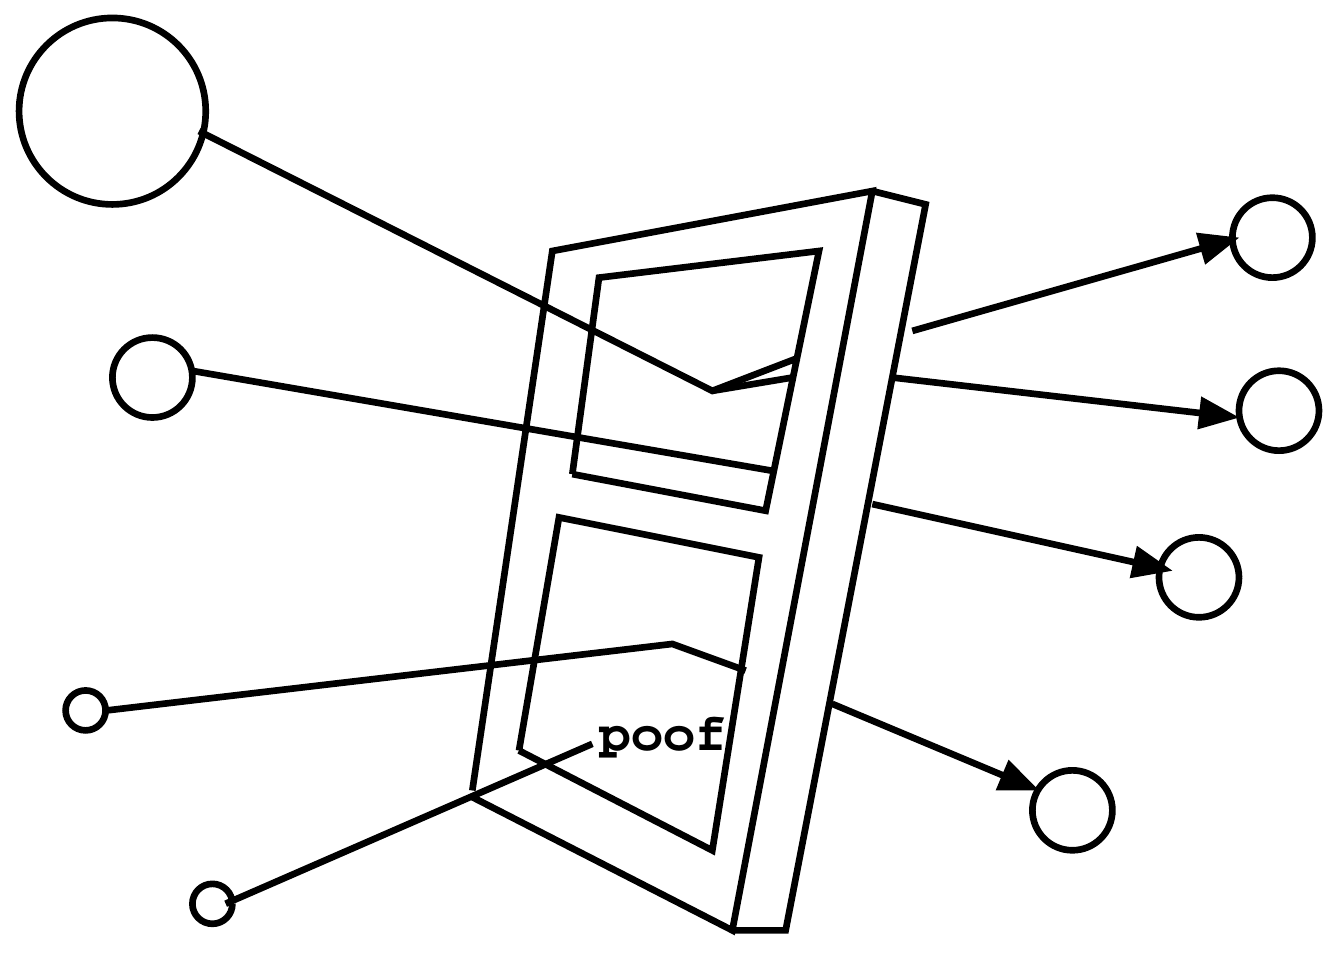
\includegraphics[width=0.5\textwidth]{./chapters/lit_review/figures/ww-mcnp.png}
  \caption[Weight window illustration]{Cartoon illustration of a weight window,
    adapted from \cite{brown_mcnp_2002, mcnp_manual_v2}}
  \label{fig:ww-mcnp}
\end{figure}
%
The first particle we see entering the weight window is a single, high-weight
particle. The weight of this particle is above the weight window bounds, so as
it enters the weight window it is split into multiple particles whose weight is
within the window bounds. The second particle entering the window is within the
weight window bounds, so it retains its weight and is not split or rouletted.
The last two particles entering the window have weights lower than the bound.
They undergo a rouletting routine and one particle is killed and the surviving
particle is increased in weight. As these particles leave the window, all of
them have weights within the range of the window. This will reduce the variance
of the particles contributing to a tally in that region. However, the user is
faced with calculating a significant number of parameters to
determine weight windows for the entire problem. In the best case with an
experienced user, this may just take time. With an inexperienced user or a
difficult problem this can
be insurmountable, and may be too difficult to do without some automated
assistance.

It should be noted that
while splitting and roulette can be performed on a single variable--energy,
space, or time--the weight window is either energy-space
dependent or space-time dependent. Further, the weight window will split or
roulette depending on the particle weight entering the window. Splitting and
roulette on their own either increase or decrease the particle weight
proportional to $I'/I$ no matter what the entering particle weight is. As a
result, poorly chosen splitting or roulette parameters on their own can still
have significant tally variance, because particle weights may still span a wide
range.

Modified sampling methods adjust transport by sampling from a different probability
distribution function than the actual distribution for the problem. This is
possible if, as with population control methods, the particle weights are adjusted
 accordingly.
 The new probability distribution function should bias particles in regions of high
 importance to the problem tallies. In MCNP, a number of modified sampling
 methods exist.
 These include the exponential transform, implicit capture, forced collisions, source
 biasing, and neutron-induced photon production biasing.

The exponential transform modifies particle transport from the analog problem by
artificially modifying the macroscopic cross section, and thus the
distrance-to-collision, to move particles in important directions. In directions
of higher importance, the cross section is reduced, and particles can flow more
freely. In directions of lower importance, the cross section is increased, and
particles more frequently interact, thereby increasing their probability of
directional change or absorption. The transformed cross section used by the
exponential transform is defined by
%
\begin{equation*}
  \Sigma_t^* = \Sigma_t(1-p\mu) ,
\end{equation*}
%
where $\Sigma_t^*$ is the transformed total cross section, $\Sigma_t$ is the
true total cross section, $p$ is the transform parameter, and $\mu$ is the
cosine of the angle between the preferred direction and the particle's transport
direction \cite{mcnp_manual_v1, mcnp_manual_v2, hendricks_mcnp_1985}.

Because the particle's transport is adjusted in the exponential transform, the
particle weight must be adjusted accordingly. This is given by
%
\begin{equation*}
  \begin{split}
  w^* &= \frac{\Sigma_t e^{-\Sigma_t s}}{\Sigma_t^* e^{-\Sigma_t^* s}} \\
      &= \frac{e^{-\rho \Sigma_t \mu s}}{1-p\mu}, \\
  \end{split}
\end{equation*}
%
where $s$ is the phase space of particle residence. This weight adjustment
ensures that the particle weight is conserved throughout transport, even as
the cross section is altered. Because the cross section in the problem is both
energy and material dependent (depending on the geometry), the exponential
transform will be dependent on space and energy, and particles will be biased in
both. While a powerful method, the exponential transform is quite difficult to
use and if $p$ is chosen poorly, this method can perform quite poorly. Further,
the user has to know quite a bit about the problem physics and material to choose an
optimal quantity for $p$.

Source biasing, rather than preferentially adjusting particles' directionality
by way of adjusting the cross sections, biases particles from their origin.
Source biasing has the option to bias particles in energy, direction, and space
(if the source is volumetric). This allows the user to choose importance
separately for each variable. First, the source variable (let us consider
energy for the moment) is defined as a series of bins or a function. Second, the bins are
assigned probabilities of occurence according to their importance. An energy bin
with a high importance will be assigned a high probability of occurence, and a
bin with low importance will be assigned a low probability of occurence. As
particles are born in the bins with higher importances, they will have their
weights adjusted to the inverse of their probability of occurence, or $w^* =
p/p^*$. Here $p$ refers to the probability density function for the source
particles; it bears no relation to the exponential transform factor.

Source biasing is a very simple method that can reduce the solution variance
significantly. However, if a user chooses bin sizes or a function that does not
properly reflect the particles importances in the problem, the source will be
poorly sampled. As a result, sampling may be very inefficient and the figure of
merit will decrease. In MCNP, if poor parameters are chosen for this method, the
user will be given a warning.

Truncation methods stop tracking particles in a region of phase-space that is of
low-importance to the tally. These methods can be used in space (a vacuum boundary
condition), energy (eliminate particles above or below a specified energy), or
time (stop
tracking after a given time). To effectively use these methods, the user must be
aware of
particles' importance to a tally result. If particles that are important to a
result are
 eliminated with a truncation method, the tally will lack the contribution from
 that particle's phase-space, and will be underestimated as a result. Further,
 as discussed in Section \ref{subsubsec:CLT}, the central limit theorem only
 holds assuming that the histories tracked are random and independent.
 Truncating particles of high importance remove the independence from the
 sampling, and the estimate of the response will be wrong.

It is important, in using any variance reduction technique, to ensure that a
fair game
is being played. The user must ensure that the fundamental nature of the problem
is not
being changed by using a variance reduction technique, or the answer will not be
representative of the original problem. Automated variance reduction techniques aim to
eliminate this uncertainty for the user by estimating the importance of
particles in some
 way and then setting up variance reduction parameters automatically.
The remainder of this literature review will focus on efforts to
automate population
control methods and modified sampling methods for variance reduction.

\subsection{Automated Variance Reduction Methods for Monte Carlo Radiation
Transport}
\label{subsec:AutomatedMCVR}

Section \ref{subsec:MCVR} described the methods that one may use to reduce the
variance in Monte Carlo radiation transport tallies. These methods, if used
correctly, can significantly increase the transport efficiency in a Monte Carlo
simulation. However, correct use of these methods often requires intelligent
selection of variance reduction parameters, which is a non-trivial task. Users
found themselves often performing several trial runs before choosing final
quantities for the VR parameters in their problems, which was computationally
inefficient and still required significant knowledge of Monte Carlo and variance
reduction to do well \cite{booth_automatic_1982}.

This has been addressed by using Monte Carlo to sample the problem in an initial
calculation to determine more favorable variance reduction parameters automatically.
Booth and Hendricks,
recognizing that choosing optimal weight window values for energy- and space-
dependent weight windows was difficult even for experienced users proposed a
Monte Carlo importance generator \cite{booth_automatic_1982} that could be used
to select weight window values automatically for a given problem
\cite{hendricks_code-generated_1982}.
The importance generator estimated a cell's importance
by tracking the weights of the particles in the cell, or
\begin{equation}
  Importance  = \frac{\text{score of particles leaving the cell}}
                     {\text{weight leaving the cell}}.
\label{eq:BoothImp}
\end{equation}
and then used these importances to select weight window parameters
\begin{equation}
  W_{i,low} = \frac{1}{kN}\big(\Sigma W_{i,in} + \Sigma W_{i,out} \big)
\end{equation}
\begin{equation}
  W_{i,high} =
  \begin{cases}
    k*W_{i,low} & \text{if } W_{i,low} \neq 0, \\
    \infty & \text{if } W_{i,low} = 0.
  \end{cases}  .
  \label{eq:hendricksWW}
\end{equation}
where $W_{i,low}$ and $W_{i,high}$ are the weight window lower and upper weight
bounds respectively, $W_{i,in}$ and $W_{i,out}$ are the total weight entering
and leaving the cell, $N$ is the number of source particles, and $k$ is some weight
window width (a constant). In his
paper, Booth notes that the weight window target value was chosen so that the
track weight times the expected score in the tally region (for unit track
weight) was approximately constant. Booth's importance generator saw
improvements in the FOM between 1.5-8x when compared to the analog run for the
test problem presented. Booth and Hendricks combined these two methods to
automate weight window generation based on phase-space importance
\cite{booth_deep_1982, booth_importance_1984}. They showed that the combination
of the importance estimator and the weight window generator was a successful way
to perform variance reduction in deep-penetration problems. However, their
method depended on several iterations of importance-determining runs to obtain a
satisfactory estimation of the importance. For a 300cm slab problem, the FOM was
increased from 1.9 to 75, but took 10 subsequent runs to obtain the FOM of 75,
and these runs ranged from 1.2 min (for the analog problem) to 42 minutes (for
the 9th run \cite{booth_importance_1984}.

It should be noted that both the importance generator and the weight window
generator use a lower-quality
Monte Carlo run to gain an initial estimate for a cell's importance and generate
variance reduction parameters from them to bias a more computationally-intensive
run. Naturally, the variance reduction parameters generated by using these
techniques are limited by the statistical precision in the regions used to
generate them. Hendricks also pointed out that the weight window generator
tended to populate all regions of phase space equally, which he conceeded was
not ideal for all problems \cite{hendricks_code-generated_1982}.
Furthermore, for deep-penetration particle transport, the
variance reduction parameters for low flux regions are exceedingly difficult to
generate, resulting in unfavorable VR parameters.

The MCNP \cite{mcnp_manual_v1, brown_mcnp_2002} weight window generator has been
extended beyond the initial space- and energy- implementation described in
booth's paper. It now has the ability to automatically generate space- energy-
and angle- weight windows. The importance generator in MCNP also has been
extended to time-importance, and those values can be used for splitting or
roulette parameters \cite{brown_mcnp_2002}, and can be optimized on a grid
independent from the MCNP geometry \cite{evans_enhanced_1998}.
It As with Booth and Hendricks'
original implementations, this updated weight window generator still relies on
adequate sampling to obtain sufficient weight window parameters. When additional
degrees of freedom, like angle-dependence, are added, this means that the time
to converge on those parameters will take even longer. The weight window
generator also only allows for a single tally to be optimized at once, so
multiple tallies cannot be optimized simultaneously. Last, the weight window
generator still requires user input and updating to seed the weight
window solution. The user must choose the meshing of the problem and have some
intuition as to how the problem should be subdivided. Depending on user
experience, the weight window generator can have differences in the FOM from 2
to 10 times \cite{van_riper_generation_1995}.


\section{Importance Functions for Variance Reduction}
\label{sec:Importance}

The effective use of variance reduction techniques can lead to a faster time to
a desired solution and a reduced variance in the specified tally. However,
specifying variance reduction parameters is not always a straightforward
procedure. In simple geometries, a user might intuitively understand which
regions of a problem may contribute more to a desired solution, but for more
complex geometries, this may not be so obvious.
In the following subsections, the theory in determining which regions of a
problem are important to eliciting a tally response will be described.
The first topic discussed will be
the concept of importance and obtaining a measure of importance with
Monte Carlo sampling.
Second, the adjoint equation and its relation to importance will be introduced.
Last, the contributon solution and how its relation to tally responses is
reviewed.

\subsection{The Concept of Importance}
\label{sec:Importance}

The concept of importance is, in essence, a means of defining which regions of
a problem that are likely to contribute to a
response and which are less likely to contribute to a response. The regions
that are more likely to generate a response will have a
higher importance than those that do not.
If an importance
function for a system can be obtained computationally, that importance
function can be
strategically used in variance reduction techniques to speed up the Monte Carlo
calculations.

As described in Section \ref{subsec:AutomatedMCVR}, Booth
\cite{booth_automatic_1982} proposed
a method to quantify a cell's importance within a Monte Carlo simulation
(Eq. \eqref{eq:BoothImp}). In
this method, Booth suggested estimating the cell's importance using Monte Carlo
transport as:
\begin{equation*}
  Importance  = \frac{\text{score of particles leaving the cell}}
                     {\text{weight leaving the cell}}.
\end{equation*}
This particular calculation of importance
follows from the intuitive explanation for importance in the preceding
paragraph. Recall from Section \ref{subsec:MCVR} that in variance reduction
methods, the population of particles is increased in important regions such that
the number of samples or particles contributing to a tally increases, but the
total problem weight is conserved. More important regions should have many
lower-weight particles to reduce the tally variance. Using Booth's bookkeeping
method for estimating regional importance,
if a cell has a greater weight leaving the cell than the number
of particles, that means that the relative contribution of that cell to the
tally is likely to be lower than other regions. If, instead, the number of
particles leaving the cell is greater than the weight leaving the cell, then
that region is more important to the tally response, because that particle
population is higher than other cells.

While this
estimation of the importance requires only a Monte Carlo forward calculation of
the problem, it was referred to as the forward-adjoint importance generator
\cite{booth_automatic_1982, booth_deep_1982, booth_importance_1984} because the
bookeeping tracked by Eq. \eqref{eq:BoothImp} was a forward-approximation of the
adjoint. Adjoint theory and how it relates to importance will be discussed in
Section
\ref{sec:AdjointImportance}.
Booth's estimation of importance was used to generate
weight window target values inversely proportional to the importance.
In this case, the track weight times the expected score is approximately
constant in the problem. Choosing this inverse relationship between the weight
window and importance is common practice in variance reduction, and is often a
good choice because it is nearly optimal over a broad range of a problem
phase-space \cite{booth_common_2012}.

It should be noted that Booth's method is reliant on the statistical
precision of the cells sampled to generate their importances. For
deep-penetration problems, obtaining a ``good'' estimate of the cell importances
many mean free paths from the forward source takes several iterations. With
large fluctuations between iterations, this has the potential to
be a very slow and
computationally inefficient way to calculate importance in a problem. Using a
solution of the adjoint that is equally valid across all of the problem space
is more ideal for deep-penetration problems.

\subsection{The Adjoint Solution for Importance}
\label{sec:AdjointImportance}

Using the solution of the adjoint formulation of the neutron transport
equation is one of the most widely recognized methods for generating
an importance function. This subsection will begin with a brief summary of
adjoint theory. A discussion on how
the adjoint solution differs physically from the forward solution for a
particular problem follows. Last, some early investigations on how the
adjoint
and importance are related are summarized.

\subsubsection{Theory}

In previous sections we have reviewed the statistical precision of Monte
Carlo-based methods, and how sampled results in Monte Carlo can be obtained
in less time
with variance reduction methods. We have also briefly addressed the forward and
the adjoint solutions for a particular problem. In neutron transport, the
integral form of the forward, steady-state, particle transport equation can be
defined as:
\begin{multline}
\hat\Omega \cdot \nabla \psi
        (\vec {r} ,E,\:\hat\Omega)+\Sigma _{ t }
        (\vec{r},E)\psi (\vec { r } ,E,\:\hat\Omega) = \\
        \int _{ 4\pi  } \int _{ 0 }^{ \infty  } \Sigma _{ s }(E'\rightarrow E,
        \hat\Omega'\rightarrow\hat\Omega)\psi (\vec { r } ,E',\: \hat\Omega')dE'
        \:d\hat\Omega' + q_{e}(\vec { r } ,E, \:\hat\Omega),
\label{eq:F-NTE}
\end{multline}
where $\vec { r }$, $E$, and $\hat\Omega$, are direction, energy, and angle,
respectively, giving six dimensions of phase-space in total.
$\psi$ is the neutron flux, $\Sigma$ is the neutron
interaction (scattering, absorption, total) cross section, and $q_{e}$ is the
external fixed source. Alternatively, this can be written in operator form,
\begin{equation}
  H \psi = q_{e} \:,
\label{eq:F-NTE2}
\end{equation}
where $H$ represents the streaming, scattering, and absorptive terms from Eq.
\eqref{eq:F-NTE}, $\psi$ is the angular flux as it is in Eq. \eqref{eq:F-NTE}, and
$q_{e}$ is the source term.

The forward transport equation tells us where particles are moving
throughout the system. Of note: the
particles move in the scattering term from $E'$ into $E$, and from $\hat\Omega'$
into $\hat\Omega$. Therefore, for a particular problem with a given $q_{e}$,
particles start at $q_e$ and move throughout the system,
either downscattering in energy, streaming out of the problem,
absorbed by the problem materials, or
induce a response at the tally location.

The adjoint equation of the same form, in contrast, can be expressed as:
\begin{multline}
-\hat\Omega \cdot \nabla \psi^{\dagger}
        (\vec {r} ,E,\:\hat\Omega)+\Sigma _{ t }
        (\vec{r},E)\psi^{\dagger}  (\vec { r } ,E,\:\hat\Omega)
       = \\
        \int _{ 4\pi  } \int _{ 0 }^{ \infty  } \Sigma _{ s }(E\rightarrow E',
        \hat\Omega\rightarrow\hat\Omega')\psi^{\dagger}  (\vec { r } ,E',\:
        \hat\Omega')dE' \:d\hat\Omega' + q_{e}^\dagger(\vec { r } ,E,
        \:\hat\Omega),
\label{eq:A-NTE}
\end{multline}
or in operator form as
\begin{equation}
  H^{\dagger} \psi^{\dagger} = q_{e}^{\dagger},
\label{eq:A-NTE2}
\end{equation}
where the variables with $\dagger$ signify the adjoint-specific variables for
the problem: the adjoint flux $\psi^{\dagger}$ and the adjoint source
$q_{e}^{\dagger}$.
Note here that the particles in the adjoint equation move from $E$ into $E'$, and
from $\hat\Omega$ into $\hat\Omega'$, which indicates an upscattering in energy
and a reversal of direction when compared to the forward problem.
The external source, too, is different, changing
from $q_{e}$ to $q_{e}^\dagger$.

To solve the adjoint problem the adjoint source, $q_{e}^{\dagger}$,
can be chosen such that it has the potential to reveal information about the
forward problem. In MC variance reduction, we seek to obtain
information on the
detector or tally response for the system.
The response for the forward problem
given a defined source distribution  $q(\vec{r}, E, \hat{\Omega})$ is
\begin{subequations}
\begin{equation}
  R_{tally} = \int_{4\pi} \int_{V} \int_{E} \psi(\vec{r}, E, \hat{\Omega})
  \Sigma_{tally}(\vec{r},E, \hat\Omega) dE dV d\hat\Omega ,
\end{equation}
where $dE$ $dV$ and $d\Omega$ are the differential spaces of energy, volume, and
angle in the tally region.
This can be simplified using bracket notation, where the brackets indicate an
integration over all phase-space,
\begin{equation}
  R_{tally} = \langle \psi \Sigma_{tally} \rangle .
\end{equation}
\end{subequations}
$\psi$ is the angular flux and $\Sigma_{tally}$ is the effective tally
response function.

For a simple source-detector problem, we choose
$q_{e}^{\dagger}$ to be $\Sigma_{tally}$; or the adjoint source is the
tally/detector response function
for the system. Therefore, the adjoint particles start at low energy at the detector
location, move away from the adjoint source (the detector location), and scatter
up in energy. By making the choice that $q_{e}^{\dagger} = \Sigma_{tally}$, the
response function can be written as a product for the forward flux and the
adjoint source
\begin{equation}
  R_{tally} = \langle \psi q^{\dagger} \rangle .
  \label{eq:response1}
\end{equation}
By using the adjoint identity and the same operators $H$ from Eqs. \eqref{eq:F-NTE2}
and \eqref{eq:A-NTE2}
\begin{equation}
  \langle \psi, H^{\dagger} \psi^{\dagger} \rangle =
  \langle \psi^{\dagger}, H \psi \rangle .
\end{equation}
Eq. \eqref{eq:response1} can be written as a function of the
adjoint flux and the forward source distribution
\begin{equation}
  R = \langle \psi^{\dagger} q \rangle .
  \label{eq:response2}
\end{equation}

At this point, we know that the solution to the adjoint problem
transports particles from the adjoint source (which is the detector or tally
location) into the problem phase-space. The adjoint particles are
upscattered in energy and are transported in $-\Omega$ relative to the forward
problem. However, it may not be immediately obvious how this adjoint solution
relates to importance for the forward solution. Let us start with a simple
illustrative example: a monoenergetic, monodirectional, point source. The
forward source takes the form of a delta function:
\begin{equation*}
  q(\vec{r}, E, \hat{\Omega}) = \delta(\vec{r}-\vec{r}_0) \delta(E-E_0)
  \delta(\hat{\Omega}-\hat{\Omega}_0) .
\end{equation*}
Using this definition of the forward source and evaluating Eq.
\eqref{eq:response2}, we obtain
\begin{equation*}
  \begin{split}
    R &= \langle \psi^{\dagger} q \rangle \\
    &= \int_{V} \int_{E} \int_{\Omega} \psi^{\dagger}(\vec{r}, E, \hat{\Omega})
       q(\vec{r}, E, \hat{\Omega}) d\hat\Omega dE dV \\
       & = \psi^{\dagger}(\vec{r}_0, E_0, \hat{\Omega}_0).
\end{split}
\end{equation*}

This result shows that the solution to the adjoint equation is the detector
response for the forward problem. As a result, the adjoint flux can be used as
an indicator of a particle produced in $\vec{r}, E, \hat{\Omega}$ contributing
to a response in the system. This indicator can be thought of as the particle's
importance to achieving the tally or response objective. Consequently, it is
often said that the adjoint is the importance function for the problem.

The adjoint solution is used in nuclear engineering for a number of
applications, including reactor physics and perturbation theory
\cite{lewins_importance_1965, lewins_developments_1968,
greenspan_developments_1976, lux_monte_1991}.
However, Goertzel and Kalos' early work recognized its
application for deep-penetration radiation shielding.
Goertzel and Kalos \cite{goertzel_monte_1958}
showed analytically
that the exact adjoint solution, if used as an importance or weighting
function for the forward Monte Carlo calculation, will result in a zero variance
solution for the forward Monte Carlo problem. Further, Kalos
\cite{kalos_importance_1963} showed in a 1D infinite hydrogen slab problem that
an analytically-derived adjoint importance function significantly improved the
speed to convergence for neutron
transport in deep-penetration problems.

Goertzel and Kalos' finding that an exact adjoint can lead to a zero variance
solution means that if a single particle is transported with the adjoint
weighting function, its score will be the same as the total system response.
Only a single particle is required to get an exact solution for the forward
problem. This is prohibitive because obtaining
an exact adjoint solution is just as computationally expensive as getting
an exact forward solution. Instead, one seeks to obtain a good, but fairly
inexpensive, estimate of the
adjoint solution based on computational limitations. A good importance estimate
should help reduce the variance in a reasonable amount of time and be
relatively computationally inexpensive. A Monte Carlo solution can
provide a continuous solution over the problem phase-space. However, as
discussed in Section \ref{subsec:MCVR}, the quality of this adjoint solution
relies on the number of samples used to calculate it and that may take a
significant amount of time. A deterministic solution
has the potential to offer equal or better solution confidence across the
entire problem. However, it is discretized in space, energy, and angle.
For deep-penetration importance functions, we
opt for deterministically-obtained solutions due to the solution's equally
distributed validity.

\subsubsection{Implementation}

Coveyou, Cain, and Yost \cite{coveyou_adjoint_1967} expanded on Goertzel and
Kalos' work by interpreting in which ways the adjoint solution could be adapted
for Monte Carlo variance reduction. In particular, they investigated the choice
of biasing schemes and how effective they were at variance reduction for a
simple one-dimensional problem. They reiterated that the adjoint solution is a
good estimate for importance, but should not be calculated explicitly, and
rather estimated by a simpler model. The adjoint function is not necessarily the
most optimal importance function; however, it is likely the closest and most
obtainable estimate of importance that can be calculated
\cite{coveyou_adjoint_1967}. They
concluded that source biasing by the solution to the adjoint equation or by the
expected response is the best choice for Monte Carlo variance reduction, as it
can be used independently from any other variance reduction technique, and
provides good results.

Tang and Hoffman \cite{tang_monte_1988} built off of the parameters derived by
Coveyou et al.\ \cite{coveyou_adjoint_1967} to generate variance reduction
parameters automatically for fuel cask dose rate analyses. In their work, Tang
and Hoffman used the 1D discrete ordinates code XSDRNPM-S to
calculate the adjoint fluxes for their shielding problems. The results from this
calculation were then used to generate biasing parameters for Monte Carlo;
specifically, they aimed at generating parameters for energy biasing, source
biasing, Russian roulette and splitting, and next event estimation
probabilities. They implemented their work in the SAS4 module in SCALE
\cite{SCALE6_1}; it was
one of the earlier implementations of a fully-automated deterministic
biasing procedure for Monte Carlo.

\subsection{The Contributon Solution for Importance}
\label{sec:ContributonImportance}

Contributon theory is another useful concept that can be used as a measure of
importance
\cite{williams_generalized_1991,williams_contributorn_1992,williams_contributon_study}.
However, contributon theory quantifies importance differently than
adjoint theory. In contributon transport, a pseudo-particle, the
\textit{contributon}, is defined. The contributon carries response in the problem
system from the radiation source to a detector. The
total number of contributons in a system are conserved by the \textit{contributon
conservation principle}: all contributons that are emitted from the source
eventually arrive at the detector. Much of the work in this realm has been done
by Williams and collaborators
\cite{williams_generalized_1991,williams_contributorn_1992,williams_contributon_study}.

The contributon transport equation can be derived in a form analogous
to the forward (Eq. \eqref{eq:F-NTE}) and adjoint (Eq. \eqref{eq:A-NTE}) equations.
The derivation of Eq. \eqref{eq:Cont-NTE} and its corresponding variables is
available in a number of the sources referenced in this section, so we will
abstain from re-deriving it here. The angular contributon flux is defined
as the product of the forward and
adjoint angular fluxes:
\begin{equation}
\Psi (\vec {r} ,E,\:\hat\Omega) = \psi^{\dagger} (\vec {r} ,E,\:\hat\Omega)
        \psi(\vec {r} ,E,\:\hat\Omega) \:.
\label{eq.Cont-Flux}
\end{equation}
The contributon transport equation is:
\begin{multline}
\hat\Omega \cdot \nabla \Psi (\vec {r} ,E,\:\hat\Omega)
+\widetilde{\Sigma} _{ t }(\vec{r},E,\:\hat\Omega)\Psi (\vec { r } ,E,\:\hat\Omega)
     = \\
        \int _{ 4\pi  } \int _{ 0 }^{ \infty  }
        \widetilde{p}(\vec{r}, \hat\Omega'\rightarrow\hat\Omega, E'\rightarrow E)
        \widetilde{P}(\vec{r}, \hat\Omega',E')
        \widetilde{\Sigma} _{ t }(\vec{r}, E', \hat\Omega')
        \Psi (\vec { r } ,E',\: \hat\Omega')dE' \:d\hat\Omega'
        + \hat p(\vec { r } ,E, \:\hat\Omega) R .
\label{eq:Cont-NTE}
\end{multline}
The units of phase-space are the same as observed in the forward and adjoint
transport equations. The symbols decorated with tildes denote variables that are
unique to the contributon equation; $\widetilde{p}$ and $\widetilde{P}$ are both
probability functions related to scattering and $\widetilde{\Sigma}$ are
effective cross sections.
The effective cross sections are given by:
\begin{equation}
\begin{aligned}
\widetilde{\Sigma}_{t}(\vec{r}, E, \hat\Omega) &=
        \widetilde{\Sigma}_{s}(\vec{r}, E, \hat\Omega) +
        \widetilde{\Sigma}_{a}(\vec{r}, E, \hat\Omega)    \\
     &= \frac{\iint \Sigma_{s}(\vec{r},\hat\Omega''\cdot\hat\Omega,
         E\rightarrow E'') \psi^{\dagger}
         (\vec{r}, \Omega'', E'') d\Omega'' dE''}
         {\psi^{\dagger}(\vec{r}, E, \hat\Omega)}
        + \frac{Q^{\dagger}(\vec{r}, E, \hat\Omega)}
        {\psi^{\dagger}(\vec{r}, E, \hat\Omega)}.
\end{aligned}
\end{equation}
Note here that the effective scattering and absorption cross sections are
adjoint flux-dependent. Where the adjoint flux becomes small, the interaction
probabilities will become large. As a result, regions where the adjoint flux
is high interaction probabilities become low, causing fewer interactions and
more streaming. Conversely, regions with low adjoint
fluxes--like the problem boundary--will have a very high cross section, thus
encouraging particle transport back towards the adjoint source. This
increased probability of interaction in low flux regions encourages response
particle (contributon)
transport towards the detector or tally, thus contributing to a response.

The scattering probability of a contributon at position $\vec{r}$, $E'$, and
$\hat\Omega'$ is:
\begin{equation}
\widetilde{P}(\vec{r}, \hat\Omega',E') =
         \frac{\widetilde{\Sigma}_{ s }(\vec{r}, E', \hat\Omega')}
       {\widetilde{\Sigma}_{ t }(\vec{r}, E', \hat\Omega')} \:,
\end{equation}
and the probability that a contributon scattering at $\vec{r}$, $E'$,
and $\hat\Omega'$ will scatter into $d\hat\Omega$ $dE$ is
\begin{equation}
\widetilde{p}(\vec{r}, \hat\Omega'\rightarrow\hat\Omega, E' \rightarrow E) =
       \frac{\Sigma_{s}(\vec{r}, \hat\Omega'\cdot\hat\Omega, E'\rightarrow E)
       \psi^{\dagger} (\vec{r}, E, \hat\Omega)}
       {\iint \Sigma_{s}(\vec{r},\hat\Omega'\cdot\hat\Omega'',E'\rightarrow
       E'')\psi^{\dagger} (\vec{r}, E'', \hat\Omega'')d\hat\Omega'' dE''}.
\end{equation}
The distribution function governing the contributon source is
\begin{equation}
\hat p(\vec{r}, E, \hat\Omega) =
\frac{\psi^{\dagger}(\vec{r}, E, \hat\Omega) Q(\vec{r},E,\hat\Omega)}
     {\int \int \int \psi^{\dagger}(\vec{r'},E',\hat\Omega')
     Q(\vec{r'},E',\hat\Omega') d\hat\Omega' dE' dV'},
\end{equation}
note that the contributon source is actually defined in Eq.
\eqref{eq:Cont-NTE} by the product of $\hat{p}$
and $R$. $R$ is contributon production rate; it
is given by integral of the adjoint flux and the forward source
\begin{equation}
  \begin{split}
R &= \int \int \int \psi^{\dagger}(\vec{r},E,\hat\Omega)Q(\vec{r},E,\hat\Omega)
    d\hat\Omega dE dV \\
  & = \langle \psi^{\dagger}Q  \rangle
\end{split} \:,
\end{equation}
which is recognizable as the system response described
in Section \ref{sec:AdjointImportance}. It can also be shown by integrating Eq.
\eqref{eq:Cont-NTE} over all phase space and ensuring that the function
$\hat{p}$ is normalized, that
\begin{equation}
  R = \langle \widetilde{\Sigma}_a \Psi \rangle,
  \label{eq:contribprod}
\end{equation}
or the rate at which contributons die in the detector is the same as
the rate at which they are produced by the contributon source.
Knowing that $R$ is the contributon production rate, let us consider the
probability that a particle will be absorbed in the detector, or $P$, given by
\begin{equation}
  P  = \langle \Sigma_a \psi \rangle.
\end{equation}
Adding a factor of $\psi^{\dagger}/\psi^{\dagger}$ to the terms on the right hand
side, this becomes
\begin{equation}
  P = \Big \langle \frac{\Sigma_a}{\psi^{\dagger}} \psi \psi^{\dagger} \Big
  \rangle.
\end{equation}
By using the identities from the contributon equation, this is also
\begin{equation}
  P = \langle \widetilde{\Sigma_a} \Psi \rangle .
\end{equation}
Next, substituting the definition from Eq. \eqref{eq:contribprod} into this
equation, it follows that
\begin{equation}
  P = R.
  \label{eq:PR}
\end{equation}
This is the same
\textit{contributon conservation principle} introduced at the beginning of this
section.
Williams noted that one could
go so far as to transport contributons rather than real particles with Monte Carlo.
Because every particle transported would eventually reach the detector and give
an exact value for R (as shown by Eq. \eqref{eq:PR}), this
would lead to a zero variance solution. However, the nature of solving the
contributon equation with Monte Carlo (or any other transport mechanism)
involves knowing the exact solution to the adjoint equation, and so relies on
the same computational obstacles as solving the adjoint transport equation.

As mentioned in the previous section, the adjoint flux is an indicator of a
particle's importance to inducing a response. Conversely, the contributon
flux describes the importance of a particle to the solution.
Becker's thesis \cite{becker_hybrid_2009} aptly points out that this is
illustrated most dramatically in a source-detector problem, where the forward
source has little importance to the adjoint source, but does have importance to
the problem solution. As a result, both the contributon solution and the adjoint
solution can be considered importance functions for a problem, but the
importance that they describe differs.

Williams recognized the applications of contributons to
shield design and optimization in an extension of contribution theory called
spatial channel theory. In particular, Williams noted that variables
relevant to contributon response were useful in determining transport paths
through media \cite{williams_contributon_study, williams_SCC_shielding}. A study
of different contributon values throughout the system could enlighten users on
regions with higher response potential. This could then be used to intelligently
choose regions for detector locations or add to shielding.
The contributon values in this theory include the contributon flux, the
contributon density, the contributon current, or the contributon velocity
\cite{williams_relations_1977}.
In this way, the
user could find the particles most influential to the response of the system. A
region with high response potential is the most important to a detector tally. The
variables of response described by Williams are the response potential, the
response current, and the response vorticity \cite{williams_contributorn_1992}.

Contributon theory and spatial channel theory have been applied successfully to
shielding analyses \cite{seydaliev_contributon_2008, williams_SCC_shielding} due
to their ability to show particle flow between a source and response effectively.
Williams and Engle showed that
spatial channel theory can be used in reactor shielding analyses.
In their work, they used
contributon currents to determine preferential flow paths through the Fast Flux
Test Facility (FFTF) \cite{williams_SCC_shielding}.
Seydaliev \cite{seydaliev_contributon_2008} used angle-dependent forward and
adjoint
fluxes and currents to visualize the contributon flux for
simple source-detector problems. In this work, he showed that contributon flow
in the system behaves much like a fluid between the source and detector,
following preferential flow paths more densely.
Seydaliev also observed ray effects in the
contributon flux for high energy photons, and traditional methods like using a
first collision source, did not remedy the issue. The contributon formulation of
particle transport can show important particle flow paths between a source and a
detector, but it is still not immune to computational obstacles that exist for
standard forward- and adjoint- transport.

The past few subsections have described the different means by which importance
can be defined or quantified for a problem.
As discussed in Section \ref{sec:Importance}, generating an importance function
with Monte Carlo is limited in that the quality of the importance map is only as
good as the regions that are sampled. For deep-penetration problems, it may be
prohibitively difficult to obtain adequate importance sampling with traditional
Monte Carlo methods.

Deterministically-obtained importance functions, however,
offer the benefit of a solution that is equally valid across all of the problem
solution-space. This is because the deterministic solution's precision is
limited to convergence criteria, not sampling of individual particles. Using a
deterministic solution is often faster and much less computationally-intensive
than Monte Carlo for importance quantification.
As a result, many hybrid methods opt
to use deterministically-obtained importance functions to generate variance
reduction parameters for Monte Carlo transport.

\section{Automated Variance Reduction Methods for Local Solutions}
\label{sec:localVR}

The next several sections (\ref{sec:localVR} through \ref{sec:AngleVR})
describe different ways that deterministically-obtained importance
functions
can be applied to variance reduction methods in practice. Local variance
reduction methods are those that optimize a tally response in a localized region
of the problem phase-space. These types of problems may be the most immediately
physically intuitive to a user,
where a person standing $x$ meters away from a source may wish to know their
personal dose rate. In this section, notable
automated deterministically-driven variance reduction methods that
have been designed for such localized response optimization are described.
Recall that Booth's importance generator (Section \ref{subsec:AutomatedMCVR})
was also designed for localized tally results, but will not be elaborated upon
here.

\subsection{CADIS}
\label{sec:CADIS}

In 1997, Haghighat and Wagner introduced the Consistent Adjoint-Driven
Importance Sampling method (CADIS)
\cite{wagner_automatic_1997,wagner_automated_1998,haghighat_monte_2003} as a
tool for automatic variance reduction for local tallies in Monte Carlo. CADIS
was unique in that it used the adjoint solution from a deterministic simulation to
consistently bias the particle distribution and particle weights. Earlier
methods had not ensured the consistency between source biasing and particle
birth weights. CADIS was applied to a large number of application problems and
performed well in reducing the variance for local tallies
\cite{wagner_review_2011}.

The next several paragraphs present and discuss
the theory supporting CADIS. Note that the theory presented is specific to
space-energy CADIS, which is what is currently implemented in existing software.
The original CADIS equations
are based on space and energy ($\vec{r}, E$) dependence, but not angle, so
$\phi^{\dagger}$ can be used rather than $\psi^{\dagger}$. This does not mean
that CADIS is not applicable to angle. This is merely a choice made by the
software and method developers given the computational resources
required to calculate and store
full angular flux datasets, and the inefficiency that using angular fluxes might
pose for problems where angle dependence is not paramount.

In trying to reduce the variance for a local tally, we aim to encourage particle
movement towards the tally or detector location. In other words, we seek to
encourage particles to induce a detector response while discouraging them from
moving through unimportant regions in the problem.
Recall from  Eqs. \eqref{eq:response1} and \eqref{eq:response2} that the total
system response can be expressed as either an integral of $\psi^{\dagger}\: q_{e}$
(the adjoint flux and the forward source), or $\psi\: q_{e}^{\dagger}$
(the forward flux and the adjoint source).
Also recall that the adjoint solution is a measure for
response importance.

\begin{subequations}
\label{CADISmethod}
To generate the biased source distribution for the Monte Carlo calculation,
$\hat{q}$,
should be related to its contribution to inducing a response in the tally or
detector. It follows, then, that the biased source distribution is the ratio of
the contribution of a cell to a tally response to the tally response induced
from the entire problem. Thus, the biased source distribution for CADIS
is a function of the adjoint scalar
flux and the forward source distribtion $q$ in region $\vec{r}, E$,
and the total response $R$
\begin{equation}
\begin{split}
\hat{q}  & = \frac{\phi^{\dagger}(\vec {r} ,E)q(\vec {r}
,E)}{\iint\phi^{\dagger}(\vec {r} ,E)q(\vec {r} ,E) dE d\vec{r}} \\
         & = \frac{\phi^{\dagger}(\vec {r} ,E)q(\vec {r} ,E)}{R}.
\end{split}
\label{eq:weightedsource}
\end{equation}
The  starting weights of the particles sampled from the biased source
distribution ($\hat{q}$) must be adjusted to account for the biased source
distribution. As a result, the starting weights
are a function of the biased source distribution and the
original forward source distribution:
\begin{equation}
\begin{split}
w_0  & = \frac{q}{\hat{q}} \\
     & = \frac{R}{\phi^{\dagger}(\vec {r} ,E)}.
\end{split}
\label{eq:startingweight}
\end{equation}
Note that when Eq. \eqref{eq:weightedsource} is placed into Eq.
\eqref{eq:startingweight}, the starting weight is a function of the total
problem response and the adjoint scalar flux in $\vec{r}, E$.
The target weights for the biased particles are given by
\begin{equation}
\hat{w} = \frac{R}{\phi^{\dagger}(\vec {r} ,E)},
\label{eq:WW}
\end{equation}
\end{subequations}
where the target weight $\hat{w}$ is also a function of the total response and
the adjoint scalar flux in region $\vec{r}, E$.
The equations for $\hat{w}$ and $w_0$ match; particles are born at the same weight
of the region they are born into. Consequently, the problem limits
excessive splitting
and roulette at the particle births, in addition to consistently biasing the
particle source distribution and weights. This is the ``consistent'' feature of
the CADIS method.

CADIS supports adjoint theory by showing that using the adjoint solution
($\phi^{\dagger}$) for variance reduction parameter generation successfully
improves Monte Carlo calculation runtime. CADIS showed improvements in the FOM
when compared to analog Monte Carlo on the order of $10^2$ to $10^3$,
and on the order of five
when compared to ``expert'' determined or automatically-generated weight
windows \cite{wagner_automated_1998, wagner_automated_2002} for simple shielding
problems. For more complex
shielding problems, improvements in the FOM were on the order of $10^1$
\cite{wagner_automatic_1997, wagner_automated_1998}. Note that CADIS improvement
is dependent on the nature of the problem and that these are merely illustrative
examples.

\subsection{Becker's Local Weight Windows}
\label{sec:beckerlocal}

Becker's work in the mid- 2000s also explored generating biasing parameters for
local source-detector problems \cite{becker_hybrid_2009}. Becker noted that in
traditional weight window generating methods, some estimation of the adjoint
flux is used to bias a forward Monte Carlo calculation. The product of this
weight window biasing and the forward Monte Carlo transport ultimately
distributed particles in the problem similarly to the contributon flux.
In his work, Becker
used a formulation of the contributon flux, as described in Eq.
\eqref{eq.Cont-Flux} to optimize the flux at the forward detector location.
The
relevant equations are given by Eqs. \eqref{eq:beckerconributon} -
\eqref{eq:beckeralpha}.

\begin{subequations}
\label{eq.beckerlocal}
First, the scalar contributon flux $\phi^c$, which is a function of space and energy
is calculated with a product of the deterministically-calculated forward and
adjoint fluxes, where
\begin{equation}
\phi^c(\vec{r},E) = \phi(\vec{r},E) \phi^{\dagger}(\vec{r},E).
\label{eq:beckerconributon}
\end{equation}
This is then integrated over all energy to obtain a spatially-dependent
contributon flux
\begin{equation}
\tilde{\phi^c}(\vec{r}) = C_{norm}\int_0^{\infty } \phi^c(\vec{r},E) dE,
\label{eq:beckerconributonspace}
\end{equation}
where the normalization constant, $C_{norm}$, for a given detector volume,
$V_D$,
is:
\begin{equation}
C_{norm} = \frac{V_D}{\int_{V_D}\int_0^{\infty } \phi^c(\vec{r},E) dE dV}.
\end{equation}
The space- and energy-dependent weight windows are given by:
\begin{equation}
  \bar{w}(\vec{r},E) = \frac{B(\vec{r})}{\phi^{\dagger}(\vec{r},E)}\:,
\label{eq:beckerlocalww}
\end{equation}
where
\begin{equation}
B(\vec{r}) = \alpha(\vec{r}) \tilde{\phi^c}(\vec{r}) + 1 -  \alpha(\vec{r})\:,
\end{equation}
and
\newcommand{\firs}{\cfrac{\tilde{\phi}^c_{max}}{\tilde{\phi}^c(\vec{r})}}
\newcommand{\seco}{\cfrac{\tilde{\phi}^c(\vec{r})}{\tilde{\phi}^c_{max}}}
\begin{equation}
  \alpha (\vec{r}) = \bigg[ 1 + \exp \bigg( \firs - \seco \bigg) \bigg]^{-1} .
  \label{eq:beckeralpha}
\end{equation}
\end{subequations}

Becker found that this methodology compared similarly to CADIS
for local solution variance reduction
for a large challenge problem comprised of nested
cubes. The particle density throughout the problem was similar
between CADIS and Becker's local weight window. The FOMs were also relatively
similar, but were reported only with Monte Carlo calculation runtimes (meaning
that the deterministic runtimes were excluded). Note that
Becker's method requires both a forward and an adjoint
calculation to calculate the contributon fluxes, while CADIS requires only an
adjoint calculation.

\section{Automated Variance Reduction Methods for Global Solutions}
\label{sec:GlobalVR}

The previous section detailed several methods that automate variance reduction for localized tallies. However, for global solutions these methods do not work well. The global tally suffers from a large range in variance across the physical problem space, and the solution is dependent on the flux distribution throughout the problem. Here several methods are described that provide automated variance reduction for global solutions or multiple tallies. 

Cooper and Larsen developed a weight window technique to reduce the variance of Monte Carlo global solutions \cite{cooper_automated_2001}. In their work, Cooper and Larsen utilized a forward solution to the transport equation to generate paramaters for a modified Monte Carlo simulation where the particles are nearly uniformly distributed throughout the problem. By doing so, the variance in the scalar flux remained relatively constant throughout the problem, rather than rising significantly with increasing distance from the forward source. Cooper's "isotropic" weight windows dependent on $\vec{r}$ are given by:
\begin{subequations}
\label{coopers}
\begin{equation}
\bar{ww}(\vec{r}) = \frac{\phi(\vec{r})}{max \phi(\vec{r})}
\end{equation}
\begin{equation}
ww(\vec{r})_{top} = \rho \bar{ww}(\vec{r})
\end{equation}
b, the linearly anisotropic factor, is
\begin{equation}
ww(\vec{r})_{bottom} = \frac{\bar{ww}(\vec{r})}{\rho}
\end{equation}
where $\rho$ is the weight window scaling factor
\end{subequations}

In practice, Cooper's algorithm was to iteratively switch between solving the diffusion equation with transport correctors (eddington factors); a process known as quasidiffusion, and with a Monte Carlo solution. An initial quasidiffusion solution was used to generate weight windows, and then after a time the Monte Carlo solution was used to generate updated eddington factors for the quasidiffusion solution. 

Because Cooper's method depended on Monte Carlo to generate the eddington factors for the quasidiffusion problem, this method was limited by the iterative switch between the quasidiffusion solution and the Monte Carlo solution. The frequency by which this switching happens is entirely up to the user, but may drastically affect the efficiency of the method. Further, Cooper notes that we do not know at what point in time (for which number of particles N) the Monte Carlo solution becomes more accurate than the quasidiffusion solution, which is an important issue in choosing solution parameters. 

Becker's forward Method: \cite{becker_hybrid_2007}

Becker's contributon method: \cite{becker_hybrid_2009}

Van Wijk's method, like CADIS and FW-CADIS, is a variance reduction method designed to operate with little user input \cite{van_wijk_easy_2011}. 
Van Wijk et al. applied their method to a PWR facility and observed a FOM increase by a factor of $>$200. 


The Method of Automatic Generation of Importances by Calculation (MAGIC) is a global variance reduction technique \cite{davis_comparison_2011} proposed by Davis in 2011. 
Rather than using a deterministic solution to obtain an estimate of the forward flux to generate an importance map, the MAGIC method uses an analog monte carlo run with multigroup cross section data and (optionally) a high energy cut-off.
This initial analog run is used to generate initial importance map for a secondary run.
This process iterates until several monte carlo simulations are run and a finalized importance map is generated. 
In their paper, the authors compared three variants of MAGIC to FW-CADIS in ITER fusion energy systems. 
These three variants used different weight window adjustments for importances: weight windows in cells based on existing weight information, weight windows in mesh cells based on flux information, and weight windows in cells based on population density. 
Davis and colleagues concluded that the most effective method for variance reduction in their system was MAGIC's weight window in mesh based on flux information, where FW-CADIS' FOM was 65\% that of MAGIC's. 
The authors did not make it clear how many iterations were required, on average, to generate the finalized weight window map or if the time to iteratively generate importance maps were included in the FOM. 
It is unclear if only the final monte carlo simulation's runtime was used to calculate the FOM. 
Furthermore, the authors did not clearly state how the biasing parameters were calculated, other than that they used flux, population density, or weight information. 


Forward-Weighted CADIS, also developed by Hagighat and Wagner \cite{wagner_forward-weighted_2007,wagner_forward-weighted_2009,wagner_forward-weighted_2010}, utilized Cooper's concept of using a forward deterministic calculation to evenly distribute particles throughout the problem subspace. However, Wagner et al took a different approach: by using a forward deterministic estimate of the flux or desired response as the adjoint source for an adjoint calculation, biasing parameters for global responses could be calculated. The adjoint source for the adjoint calculation thus depends on the desired response for the system. The generic description for the adjoint source is given by Eq. \eqref{adjointsourcesimple} and more specific parameters are given by Eqs. \eqref{FWCadglbaldose}-\eqref{FWCadglobalflux2}: 

\begin{subequations}
\begin{equation}
{ q^{\dagger}} (P)=\frac{\sigma_d(P)}{R}
\end{equation}
\label{eq:adjointsourcesimple}

The adjoint source for the spatially dependent global dose, $\int \phi(\vec{r},E)\sigma_d(\vec{r},E) dE$:
\begin{equation}
{ q^{\dagger} }(\vec { r } ,E)=\frac { \sigma _{ d }(\vec { r } ,E) }{ \int { \sigma _{ d }(\vec { r } ,E)\psi (\vec { r } ,E,) } dE }
\end{equation}
\label{eq:FWCadglobaldose}

The adjoint source for the spatially dependent total flux $\int \phi(\vec{r},E) dE $:
\begin{equation}
{ q^{\dagger} }(\vec { r })=\frac { 1 }{ \int { \phi (\vec { r } ,E) } dE }
\end{equation}
\label{eq:FWCadglobalflux}

The adjoint source for the energy- and spatially- dependent flux $\phi(\vec{r},E)$: 
\begin{equation}
{ q^{\dagger} }(\vec { r } ,E)=\frac { 1 }{\phi (\vec { r } ,E) }
\end{equation}
\label{eq:FWCadglobalflux2}
\end{subequations}

Comparing these methods, \cite{peplow_comparison_2012} 

%
%
%----------------------------------------------------------------------------------------
% While not particularly relevant to the immediate work described in this thesis, the MS-CADIS method used a sophisticated method to generate a variance-reduced source term for 
% photon does in a shutdown system. 

%However, MS-CADIS, like CADIS and FW-CADIS, employs exclusively energy- and space- based variance reduction methods. As a result, it still suffers from similar behaviors as CADIS and FW-CADIS in strongly anisotropic systems. 

%MS-CADIS \cite{ibrahim_multi-step_2014, ibrahim_analysis_2014}

\section{Automated Angle-Informed Variance Reduction Methods}
\label{sec:AngleVR}

In a number of problems, the angular dependence of the flux is significant enough that
biasing by space and energy, but not angle  is not
sufficient. As a result, a subset of hybrid methods were developed to incorporate some
degree of the flux anisotropy in variance reduction parameters. Without explicitly
calculating the angular flux, which is memory- and storage- intensive, methods
attempted to approximate the angular flux using other information more readily
accessible to them. These approaches broadly can be categorized as methods that
bias using population control methods (such as weight windows),
and methods that bias with modified
sampling methods (such as the exponential transform).
Initial approaches
to angular biasing focused on approximating the angular flux, $\psi$,
as a separable
function of the scalar flux and an angle-dependent multiplier.
These approximations of the flux were then used to generate biasing
parameters dependent on angle for highly angular-dependent problems.

\subsection{Angular Biasing with Population Control Methods}

\subsubsection{AVATAR}
\label{subsec:AVATAR}

The AVATAR \cite{van_riper_generation_1995, van_riper_avatarautomatic_1997}
(Automatic Variance and Time of Analysis Reduction) method generates
three-dimensional, space-, energy- and angle-dependent weight windows for Monte
Carlo by
using a relatively course-mesh and few-angle deterministic calculation in
THREEDANT, approximating the angular flux as a function of the scalar flux, and
then subsequently passing those flux values through a postprocessing
code, Justine, to generate
weight windows for MCNP \cite{mcnp_manual_v1}. The AVATAR approach to
determining the angular flux used an approximation of the angular flux based on
the maximum entropy distribution, which will be briefly summarized in the next
few paragraphs.

\subsubsection*{Information Theory}

First, for a given set of discrete values $x_i (i=1,2, \cdots n)$
that are passed to a function, $f(x)$, the expectation value of that function is given
by
\begin{equation}
  \big\langle f(x) \big\rangle = \sum_{i=1}^n p_if(x_i).
\end{equation}
For the probability distribution $p_i = p(x_i)$, $(i=1,2, \cdots n)$ the entropy of
$p$ is defined as
\begin{equation}
  H(p) = - K \Sigma_i p_i \ln p_i .
  \label{eq:entropy}
\end{equation}
where K is a positive constant. A proof that this is indeed the associated
maximal entropy associated with all $p_i$ is given in
\cite{jaynes_information_1957}.
For a continuous probability density function $p(x)$ over the interval I, the
entropy of the continuous function is
\begin{equation}
  H(p) = - K \int_I\ p(x) \ln p(x) dx .
\end{equation}
To maximize either of these distributions, while also maintaining that $\Sigma
p_i = 1$, one can use Lagrangian multipliers $\lambda$ and $\mu$
\begin{equation}
  p_i = e^{-\lambda-\mu f(x_i)} .
\end{equation}
This can be solved using
\begin{subequations}
  \begin{equation}
    \big\langle f(x) \big\rangle = - \frac{\partial}{\partial \mu} \ln Z(\mu)
  \end{equation}
  \begin{equation}
    \lambda = \ln\big[Z(\mu)\big]
  \end{equation}
  where
  \begin{equation}
    Z(\mu) = \Sigma_i e^{-\mu f(x_i)} .
  \end{equation}
\end{subequations}

Jaynes \cite{jaynes_information_1957} showing that the maximum
entropy probability distribution function corresponding to the previous
equations is given by
\begin{equation}
  p_i= \exp \big[ - \big( \lambda_0 + \lambda_1f_1(x_1) + \cdots + \lambda_m f_m(x_i) \
    \big) \big] ,
\end{equation}
and the entropy of this distribution is given by
\begin{equation}
  S_{max} = \lambda_0 + \lambda_1 \big\langle f_1 (x) \big\rangle + \cdots + \
  \lambda_m \big\langle f_m(x) \big\rangle .
\end{equation}

In this case, the constant K from Eq. \eqref{eq:entropy} has been set to 1.
The maximum entropy approach to calculating a probability distribution function
is an attractive option given limited information about that
distribution. This method's power lies in that it
deduces a function given limited information, but does not place too great of an
importance on missing or unwarranted information. Furthermore, a distribution
ascertained from this methodology will encompass all distributions with smaller
entropies that satisfy the same constraints. Thus it provides the most widely
applicable probability distribution function for the system that has been
defined.

Moskalev showed that by using the maximum entropy approach, a distribution function
could be reconstructed from a (truncated) Legendre expansion
\cite{moskalev_reconstruction_1993}. This is particularly
applicable to radiation transport, because often scattering terms are truncated
Legendre expansions. In his application, Moskalev derived a generalized form of
reconstructing a probability distribution from a truncated expansion, where the
true function represented by a Legendre polynomial series
\begin{equation}
  f(L,\mu) = \sum_{l=0}^L -\frac{2l+1}{2} f_l P_l(\mu)
\end{equation}
could be associated with an adjusted function (obtained from maximizing the
entropy of the known values)
\begin{equation}
  \tilde{f}(L,\mu) = \exp \big( \sum_{l=0}^{L} \lambda_l P_l(\mu) \big)
\end{equation}
such that
\begin{equation}
  (f,P_l) = (\tilde{f}, P_l); \quad l = 0, \cdots, L .
\end{equation}
Where $\lambda_l$ are the Lagrange multipliers, $\tilde{f}$ and $f$ are
$\epsilon \phi$, and are assumed to be a function of $\mu$ such that $f(\mu)
\geq 0, \mu \epsilon [-1, 1]$.
These generalized equations were then applied to
group-to-group scattering probability distribution functions, as well as
reconstructing a $L=3$ function. The reconstruction showed agreement except near
the extrema of $\mu$.

Walters and Wareing \cite{walters_nonlinear_1994, walters_accurate_1996} showed
that the angle-dependent source definition for a discrete ordinates transport problem
could be calculated using Moskalev's approach
\cite{moskalev_reconstruction_1993}. In their method, they used this approach to
reconstruct the source distribution of particles in each cell from the source
moments. For standard methods, the source in a cell expanded in Legendre moments is
\begin{equation}
  S_m(x) = S_{m,j}\bigg[ P_0(x) + \frac{S_{m,j}^x}{S_{m,j}}P_1(x)\bigg]
\end{equation}
where $S_{m,j}$ is the average source in cell j, direction m, $S_{m,j}^x$ is the
$P_1(x)$ moment of the source and the $P_0$ and $P_1$ are the associated
Legendre polynomials. Using a normalized source distribution $s_m(x)$ where
\begin{equation*}
  S_m(x) = s_m(x) S_{m,j},
\end{equation*}
the normalized distribution is
\begin{equation}
  s_m(x) = \big[ s_0 + s_1 P_1(x)\big]
\end{equation}
where $s_0$ and $s_1$ are the zeroth and first Legendre moments of the source.
The source distribution derived from the maximum entropy distribution was found
to be
\begin{equation}
  \tilde{s}(x) = \frac{\lambda_{1,k}}{\sinh (\lambda_{1,j})} \
  e^{\lambda_{1,j}P_1(x)} .
\end{equation}
$\tilde{s}$ has normalized Legendre moments $s_0$ and $s_1$ that match
$s_m(x)$. Because $\tilde{s}$ satisfies the information that can be obtained
about $s_m$, it can be used to reconstruct $S_m(x)$ by way of
\begin{equation}
  S_m(x) = \tilde{s}_m(x)S_{m,j}.
\label{eq:Walt_reconstruct}
\end{equation}
$\lambda_{1,j}$ can be found from
\begin{equation}
  s_1 = 3\bigg[ \coth(\lambda_{1,j} - \frac{1}{\lambda_{1,j}})\bigg] .
  \label{eq:WW_lambda}
\end{equation}
It should be noted that the same methodology that Walters and Wareing use to reconstruct the source
distribution from the source moments can be used to reconstruct the angular flux
in cells based on moments of the angular flux (i.e. the scalar flux and
current) \cite{walters_nonlinear_1994}.

In their paper, Walters and Wareing \cite{walters_accurate_1996} suggested that in place of
solving Eq. \eqref{eq:WW_lambda} for $\lambda_{1,j}$, that a rational polynomial
be used in place of it to reduce computational time. The
suggested polynomial for $0 \leq \lambda_{1,j} \leq 5$ was:
\newcommand{\lamvar}{\dfrac{s_{1,j}}{3}}
\begin{equation}
  \lambda_{1,j} =  \dfrac{2.99821 (\lamvar) - 2.2669248 (\lamvar)^2 }{1 - 0.769332
             (\lamvar) -0.519928 (\lamvar)^2 + 0.2691594 (\lamvar)^3} \\
\end{equation}
and for $\lambda \geq 5$:
\begin{equation}
  \lambda_{1,j} = \frac{1}{1-\bar\mu}
\end{equation}
A full derivation of Eq. \eqref{eq:WW_lambda} and how it satisfies the maximum
entropy requirements can be found in Appendix A of \cite{walters_accurate_1996}.

In their application, Walters and Wareing found that this method was accurate
over a fairly course mesh for the problems analyzed, and the computed fluxes
remined positive over the solution space. When compared to other methods, this
approach performed much better over coarse meshes. However, the analysis was
limited to one-dimensional problems. As mesh size grew finer, the method
performed similarly to other methods. However, near vacuum boundary conditions
$\lambda_{1,j} \rightarrow \infty$ at the cell boundary, causing issues in
calculating the flux in these cells.

\subsubsection*{AVATAR Implementation}

AVATAR used a deterministic

AVATAR built off of the methodology described by Walters and Wareing
\cite{walters_nonlinear_1994, walters_accurate_1996}, but instead of
reconstructing the source distribution inside the cell, the maximum entropy
method was used to reconstruct the angular fluxes. Thus the angular flux, $\psi$
was reconstructed with the scalar flux, $\phi$ and the current, $J$.
AVATAR avoided generating explicit angular fluxes with
THREEDANT by assuming
that the adjoint angular flux is symmetric about the average adjoint current vector,
$J^{\dagger}$ :
\begin{subequations}
\label{avatareqns}
\begin{equation}
  \psi^{\dagger}(\hat\Omega) = \psi^{\dagger}(\hat\Omega\cdot n)
  \label{eq:Av1}
\end{equation}
where
\begin{equation}
  n = \frac{J^{\dagger}}{ \left\| J^{\dagger} \right\| }.
\end{equation}
Note that $n, J, \psi,$ and $\phi$ all have implied dependence on $(\vec{r},
E)$.
The angular flux could then be reconstructed assuming that the angular flux is a
product of the scalar flux and some angle-dependent function
\begin{equation}
  \psi^{\dagger}(\hat \Omega \cdot n) = \phi^{\dagger} f(\hat\Omega \cdot n).
  \label{eq:Av2}
\end{equation}
Note that Eq. \eqref{eq:Av2} takes the form of Eq. \eqref{eq:Walt_reconstruct}.
Thus f is derived from the maximum entropy distribution:
\begin{equation}
f(\hat\Omega \cdot n) = \frac{\lambda e^{(\hat\Omega \cdot n)\lambda}}
                             {2 \sinh {\lambda} }
  \label{eq:Av25}
\end{equation}
and $\lambda$ is a function of the average cosine $\bar\mu$
\begin{equation}
\begin{split}
\lambda  & = \frac{2.99821 \bar\mu - 2.2669248 {\bar\mu}^2 }{1 - 0.769332
             \bar\mu -0.519928 {\bar\mu}^2 + 0.2691594 {\bar\mu}^3} \\
         & = \frac{1}{1-\bar\mu} \\
  \label{eq:Av3}
\end{split}
\end{equation}
for $ 0 \le \bar\mu < 0.8001$ and $0.8001 \le \bar\mu < 1.0 $, respectively.
Also, $\mu$ is given by
\begin{equation}
\bar\mu(\vec{r}, E) = \frac{\left\| J^{\dagger}(\vec{r}, E)
                     \right\|}{\phi^{\dagger}(\vec{r}, E)}.
  \label{eq:Av4}
\end{equation}
\label{eq:AvEqns}
\end{subequations}
Equations \eqref{eq:Av3} and \eqref{eq:Av4} are exact in both isotropic and
streaming conditions \cite{van_riper_generation_1995}.

Using the calculation of the angular flux described in Eqs. \eqref{eq:Av1}
through \eqref{eq:Av4}, angle-dependent weight windows could be constructed.
AVATAR's space- energy- and angle-dependent weight window is given by
\begin{equation}
\bar {w} (\vec{r},E,\hat\Omega) = \frac{k}{\phi^{\dagger}(\vec{r},E)
                                  f(\hat\Omega \cdot n)},
\end{equation}
where k is a constant that can be adjusted to match the source distribution.
In the case of AVATAR, k was used as a normalization factor to ensure that
source particles are born with weights within the weight window.
AVATAR exclusively generated weight windows, and did not attempt to consistently
bias the source
distribution. Physically, the assumption behind AVATAR is that the adjoint
angular flux
is locally one-dimensional, so azimuthal symmetry is assumed.

\subsubsection*{AVATAR Results}

The authors of AVATAR showed that AVATAR's angularly-dependent
weight windows improved the FOM (from 5- to 7-times) for a multiple-tally well-logging
problem compared to the MCNP weight window generator. AVATAR was also compared
to other methods in subsequent papers \cite{evans_enhanced_1998}. In an
update of the MCNP weight window generator, AVATAR was compared to variants of
the weight window generator and performed had a FOM of 79 while variants of the
weight window generator had FOMS ranging from 105 to 119
\cite{evans_enhanced_1998}. However, they required
multiple iterations of Monte Carlo transport to converge on weight window values
while AVATAR did not. Total runtimes for iteratively converging on weight window
values were in the 200- to 300- minute range, while AVATAR took roughly 5
minutes to converge on weight window values for the problem.

The MCNP weight window generator has also been adapted to use weight window
values seeded by a solution from AVATAR \cite{evans_enhanced_1998}. This method
had FOMs comparable to the default MCNP weight window generator, but only
required 1 iteration to converge, rather than 3. This reduced the total
transport runtime from roughly 260 minutes to 140 minutes, but still required
user experience and input to adequately set up and prepare the deterministic
input for AVATAR.

The method used by AVATAR to produce angle-dependent weight windows successfully
incorporated angular information into variance reduction parameters for Monte Carlo
with very little additional computational burden. However, because AVATAR
was not fully automated, the user had to have knowledge on the use of the $S_N$
deterministic solver in addition to the Monte Carlo methods they were trying to
optimize. As a result, the user needed to adequately prepare the deterministic
inputs, correctly specify the adjoint source for the deterministic solve, and
then pass these values to postprocessing software \cite{peplow_consistent_2012,
evans_enhanced_1998}. The FOMs reported with AVATAR did not incorporate the
additional time required for user setup and preparation of inputs, which may be
significant. Though more computationally efficient than the weight window generator,
this aspect of AVATAR may be too substantive of an obstacle for new-user
approachability. Further, it leaves more room for user-induced error.
%
%
%----------------------------------------------------------------------------------------

\subsubsection{Simple Angular CADIS}

Simple Angular CADIS \cite{peplow_consistent_2012} built off of existing
implementations
of CADIS and FW-CADIS but incorporated angular information in the
methods. Simple Angular CADIS did so without explicitly using
angular flux solutions from the deterministic solution.
This was done by reconstructing the angular flux in the same manner employed by
AVATAR and then consistently
biasing the
source distribution with the weight windows with the same methodology as CADIS
and FW-CADIS. Recall that the original
implementation of AVATAR did not have consistent source biasing.
In their work, Peplow et al. implemented their
work in MAVRIC, a hybrid methods software package distributed with the SCALE
codebase \cite{SCALE6_1}. The Simple Angular CADIS method took two different
approaches to variance reduction:
directionally-dependent weight windows with directionally-dependent source
biasing and directionally-dependent weight windows without directional source
biasing.

\subsubsection*{Theory}

The Simple Angular CADIS approach, like AVATAR, uses a reconstruction of the
angular flux derived from the maximum entropy distribution (Section
\ref{subsec:AVATAR}). In Simple Angular CADIS, the authors approximated the
angular flux such that
%
\begin{equation}
\psi^{\dagger}(\vec{r}, E, \hat \Omega) \cong \phi^{\dagger}(\vec{r}, E)
\frac{1}{2\pi} f(\hat\Omega \cdot \hat n).
\label{eq:AvAngflux}
\end{equation}
Note that this differs from AVATAR's reconstruction of the angular flux,
Eq. \eqref{eq:Av1}, by a factor of $1/2\pi$. As it was only dependent on
$\mu$, AVATAR's original approach assumed azimuthal symmetry, but did not
incorporate any factor of integration into the angular flux reconstruction. By
including the azimuthal integration factor of $1/2\pi$, this version of
$\psi^{\dagger}$ satisfies
\begin{equation*}
  \phi^{\dagger}(\vec{r}, E) = \int \phi^{\dagger} \frac{1}{2\pi} f(\hat\Omega
  \cdot \hat n) d \hat\Omega .
\end{equation*}
The corresponding angle-dependent weight windows are then given by:
\begin{equation}
\bar {w} (\vec{r},E,\hat\Omega) = \frac{2 \pi k}{\phi^{\dagger}(\vec{r},E)
                                  f(\hat\Omega \cdot n)}
\end{equation}
$f(\hat\Omega \cdot \hat n)$ is given by the same equations
\eqref{eq:Av25}, \eqref{eq:Av3}, \eqref{eq:Av4} as AVATAR.

For the variant method with directionally-dependent weight windows and without
directional
source biasing, the biasing parameters are given by Eqs. \eqref{SA-CADIS1}.
\begin{subequations}
\label{SA-CADIS1}
The biased source distribution, $\hat{q}(\vec{r},E,\hat\Omega)$,
is given by a combination of the standard CADIS
biased source, $\phi^{\dagger}(\vec{r},E)$ and the original directional
source distribution, $q(\hat\Omega \cdot \hat d)$ such that
\begin{equation}
\begin{split}
\hat{q}(\vec{r},E,\hat\Omega) & = \frac{1}{R} q(\vec{r},E) \phi^{\dagger}
                                  (\vec{r},E) \frac{1}{2 \pi} q(\hat\Omega \cdot
                                  \hat d)\\
                              & = \hat{q}(\vec{r},E) \frac{1}{2 \pi}
                              q(\hat\Omega \cdot \hat d).
\end{split}
\end{equation}
The direction $\hat d$ is sampled using the original directional source
distribution $q(\hat\Omega \cdot \hat d)$.
The birth weight matches standard CADIS with
\begin{equation}
\begin{split}
w_0  & = \frac{q(\vec{r},E,\hat\Omega)}{\hat{q}(\vec{r},E,\hat\Omega)} \\
     & = \frac{R}{\phi^{+}(\vec {r} ,E)},
\end{split}
\end{equation}
and the weight window target value is given by
\begin{equation}
\begin{split}
\bar{w} (\vec{r},E,\hat\Omega)  & = \frac{R}{\phi^{\dagger}(\vec{r},E)}
                                    \frac{f(\hat{\Omega_0}\cdot n(\vec{r_0}, E_0))}
                                    {f(\hat\Omega \cdot n)} \\
                                & = \bar{w}(\vec{r},E) \frac{f(\hat{\Omega_0}\cdot
                                    n(\vec{r_0}, E_0))}{f(\hat\Omega \cdot n)}.
\end{split}
\end{equation}
\end{subequations}
Note that the biased source distribution, $\hat{q}(\vec{r},E,\hat\Omega)$, is a
function of
the biased source distribution from traditional space- energy- CADIS and of the
original
directional source distribution; which is why this method has directional weight
windows,
but not directional source biasing.

For the second method, with directionally-dependent weight windows and with
directional
source biasing, the biasing parameters are given by the equations summarized in
Eqs. \eqref{SA-CADIS2}.
\begin{subequations}
\label{SA-CADIS2}

The biased source distribution is given by a combination of the
space-energy biased source distribution, the original directional source
distribution, and a directionally-dependent biased source distribution,
$f(\hat\Omega \cdot \hat{n_0})$ such that
\begin{equation}
\begin{split}
\hat{q}(\vec{r},E,\hat\Omega) & = \frac{1}{Rc} q(\vec{r},E,\hat\Omega)
                                  \phi^{\dagger}(\vec{r},E,\hat\Omega) \\
                              & = \left[ \frac{1}{R}q(\vec{r},E)
                                \phi^{\dagger}(\vec{r},E)
                                  \right] \left[\frac{1}{c}\frac{1}{2 \pi}
                                    q(\hat\Omega
                                  \cdot \hat d) \frac{1}{2 \pi}
                                  f (\hat\Omega \cdot n_0)\right]  \\
                             & = \hat{q}(\vec{r},E) \left[\frac{1}{c}\frac{1}{2 \pi}
                                 q(\hat\Omega \cdot \hat d) \frac{1}{2 \pi}
                                 f(\hat\Omega \cdot n_0) \right].
\end{split}
\end{equation}
The constant $c$ is given by
\begin{equation}
c = \int{\frac{1}{2 \pi} q(\hat\Omega \cdot \hat d) \frac{1}{2 \pi}
    f (\hat\Omega \cdot n_0)} d\hat\Omega.
\end{equation}
The birth weights are also a function of direction, where
\begin{equation}
\begin{split}
w_0  &= \frac{q(\vec{r},E,\hat\Omega)}{\hat{q}(\vec{r},E,\hat\Omega)} \\
     &= \frac{R}{\phi^{+}(\vec {r} ,E)} \frac{2 \pi c}{f(\hat\Omega \cdot n_0)},
\end{split}
\end{equation}
as are the target weights
\begin{equation}
\begin{split}
\bar{w} (\vec{r},E,\hat\Omega)  &= \frac{R}{\phi^{\dagger}(\vec{r},E)}
                                   \frac{2 \pi c}{f(\hat\Omega \cdot n_0)} \\
                                &= \bar{w}(\vec{r},E) \frac{2 \pi
                                    c}{f(\hat\Omega \cdot n)}.
\end{split}
\end{equation}
\end{subequations}

Details about how the aforementioned equations were practically implemented are
detailed in \cite{peplow_consistent_2012}. The motivated reader may explore this
reference for details on the calculation of $\lambda$, $\bar{\mu}$,
$\left\| J^{\dagger}(\vec{r}, E)\right\|$ and $f(\hat\Omega \cdot \hat{n_0})$

\subsubsection*{Results}

To test these two modifications of CADIS, the authors ran a number of test
problems and
compared them against standard implementations of CADIS and analog Monte Carlo
runs. For a spherical boat test problem, Simple Angular CADIS without
directional biasing improved the FOM by a factor of 2 to 3. Note that because
the source in is monodirectional, directional source biasing was not compared.
Simple Angular CADIS with- and without- directional source biasing improved the
FOM for active interrogation sample problems and for simple duct streaming
problems. They did not improve the FOMs for sample problems using a neutron
porosity tool or a gamma-ray litho-density tool.

The range in performance for
angle-dependent problems was explained by the authors as a failure of the
angular flux approximation to capture the true distribution of the angular flux.
Because Simple Angular CADIS uses the same approximation in calculating the
angular flux (Eq. \eqref{eq:AvAngflux}) as AVATAR, it is limited in the types of anisotropy
that it can capture. As a result, the biasing parameters for a problem may not
adequately reflect the flux distribution, depending on whether its behavior has
been captured effectively by the P$_1$ expansion.

The authors also noted that because the weight window is dependent on
space/energy/angle the source birth weights only matched
the weight window target value at a specific point in the weight window region.
If the weight window covered a substantial region of phase-space, this could
result in particle birth weights that do not adequately correspond to the
importance of the region that they are born into, resulting in increased runtime
and a more computationally-intensive calculation.

\subsubsection{Cooper's Weight Windows}
Cooper and Larsen, in addition to generating global isotropic weight windows
from a deterministic forward solution, as
described
in Section \ref{subsec:CooperGlobal}, also developed angle-dependent weight windows
\cite{cooper_automated_2001}. Here, the forward angular flux is calculated in a
similar
manner as the AVATAR method where the angular flux is a product of the scalar
flux and an angle-dependent function. In this case, the adjustment factor also
includes a factor of $4\pi$,
\begin{subequations}
\label{cooperangle}
\begin{equation}
  \psi(\vec{r},\hat\Omega) \approx A(\vec{r})e^{\vec{B}(\vec{r}) \cdot \hat\Omega},
  \label{eq:cooper1}
\end{equation}
where $A(\vec{r})$ and $\vec{B}(\vec{r})$ are given by:
\begin{equation}
A(\vec{r}) = \frac{\phi(\vec{r})}{4 \pi}\frac{B(\vec{r})}{sinh B(\vec{r})}
\end{equation}
\begin{equation}
  \vec{B}(\vec{r}) = B(\vec{r}) \frac{\vec{\lambda}(\vec{r})}{\left|
    \vec{\lambda}(\vec{r}) \right|}
\end{equation}
and
\begin{equation}
\lambda(\vec{r}) = coth B(\vec{r}) - \frac{1}{B(\vec{r})}.
\end{equation}
If both $A(\vec{r})$ and $\vec{B}(\vec{r})$ are inserted into the equation for
$\psi(\vec{r}, \hat\Omega)$, Eq. \eqref{eq:cooper1},
the formulation will be very similar to AVATAR's
reconstruction of the angular flux. However, Cooper's method differed from
AVATAR in the calculation of $\lambda(\vec{r})$.
Cooper noted that $\lambda(\vec{r})$ could be estimated with either the scalar fluxes
and currents from a fairly low-cost quasidiffusion calculation,
\begin{equation}
  \begin{split}
    \lambda_i(\vec{r})  & = \frac{J_i(\vec{r})}{\phi(\vec{r})} \\
                        & = \frac{1}{\Sigma_{tr}(\vec{r})\phi(\vec{r})}
                       \frac{\partial}{\partial r_j} E_{ij}(\vec{r})
                       \phi(\vec{r})
  \end{split}
\end{equation}
or with the scalar fluxes and
currents directly
from the Monte Carlo solution. Recall that $E_{ij}(\vec{r})$ is the eddington
factor described in Section \ref{subsec:CooperGlobal}.
Cooper noted that because Monte Carlo robustly
calculated
these values, it was the more optimal choice. After obtaining these values from
the deterministic calculation, Cooper's angle-dependent weight window could be
calculated with
\begin{equation}
ww_{i,j} (\hat\Omega)= \frac{\psi_{i,j}(\vec{r},\hat\Omega)} {max\phi_{i',j'}/4\pi}.
\end{equation}
\end{subequations}

As mentioned in Section \ref{subsec:CooperGlobal}, Cooper's method was limited in that it used an
iterative quasidiffusion / Monte Carlo solution to generate the biasing parameters for
the problem. This method was not automated; and the ideal frequency between iterations
was never explored. However, Cooper showed in example two-dimensional problems
that the angularly dependent weight windows
significantly improved the figure of merit as compared to analog Monte Carlo.
The distributions of the FOM and the resulting tally were also much smoother
with the approach described in their work.
Further, the
angular weight windows performed slightly better than the isotropic weight windows in
evenly distributing the particles, even in problems where the anisotropy was not
significant. However, like
AVATAR, this method is limited in the types of anisotropy it can quantify due to
the approximations it uses to reconstruct the angular flux. In generating the
estimates for $\vec{\lambda}$, the authors found that using a quasidiffusion
estimate was more efficient than using Monte Carlo estimates, likely because the
estimates of the factors could be periodically updated as the solution
iteratively converged.
%
%
%----------------------------------------------------------------------------------------

\subsection{Angular Biasing Using the Exponential Transform}

\subsubsection{Early Work}

Dwivedi \cite{dwivedi_new_1982} showed

Gupta and Dwivedi \cite{gupta_sampling_1985} showed

In 1985, Henricks and Carter \cite{hendricks_anisotropic_1985} described a
method by which
photon transport could be biased in angle with an exponential transform
adjustment factor.
In this study, the authors performed studies on three test problems with the
exponential
transform adjustment factor and with a synergistic angular bias and exponential
transform
adjustment.
In all studies, the synergistic biasing outperformed the exponential transform
adjustment
alone.
However, their method performed best in highly absorbing media.
The authors noted that this performance was due to the fact that the biasing
could be made
strong without undersampling scattering in the problem.
They also pointed out that while the weight window method was comparable in
efficiency to the
method described, their method avoided the choice of choosing importances and
weight window
values for biasing. Their method was limited to exclusively photon transport
biasing, and not
neutron transport; the authors were optimistic that the method could be extended
to neutron
transport.

\subsubsection{LIFT}

The LIFT \cite{turner_automatic_1997, turner_automatic_1997-1} method, developed by Turner and Larsen, is
a modification
of the zero variance solution (see Section \ref{sec:ContributonImportance})
that uses a deterministic calculation to
generate biasing
parameters for the exponential transform and weight window variance reduction
techniques.
First, the adjoint angular flux is approximated, piecewise continuous in space
in angle,
with the following equations:

\begin{subequations}
\label{LIFT}
\begin{equation}
\psi^{\dagger}_{g,n} (\vec{r},\Omega) \approx
                \phi^{\dagger}_{g,n}V_n \left[ \beta_{g,n}
                \frac{\sigma_{s_0,g \rightarrow g,n} b_{g,n}(\Omega)}{\sigma_{t,g,n} -
                \rho_{g,n}\cdot \Omega} e^{\rho_{g,n}\cdot (r-r_n)} \right]
\end{equation}
where the physical system is comprised of $V_n$ regions, and
$\psi^{\dagger}_{g,n}$ is the
approximation of the angular flux for group g and region n. Further, $\beta$,
the normalization
factor is given by:
\begin{equation}
\beta_{g,n} = \frac{1}{\int_{V_n} e^{\rho_{g,n} \cdot (r-r_n)} dr \int_{4\pi}
              \frac{\sigma_{s_0,g \rightarrow g,n} b_{g,n}(\Omega)}{\sigma_{t,g,n} -
              \rho_{g,n}\cdot \Omega} d\Omega}
\end{equation}
b, the linearly anisotropic factor, is
\begin{equation}
b_{g,n}(\hat\Omega) = 1 + 3\mu_{g\rightarrow g,n}\frac{\sigma_{t,g,n} -
                      \sigma_{s_0,g\rightarrow g,n}}{{\left| \rho_{g,n}
                      \right|}^2}\rho_{g,n}\cdot \Omega
\end{equation}
and the biasing parameter is given by
\begin{equation}
  \rho_{g,n} = \sigma_{t,g,n} \lambda_{g,n}
\end{equation}
\end{subequations}

The first equation in this series is an adjustment of the exponential transform.
However,
rather than relying upon an isotropic scattering law, like earlier
implementations of the exponential transform, the LIFT
method adjusts the transform to instead be linearly anisotropic in angle. The
parameters
$\beta_{g,n}$, $b_{g,n}$ and $rho_{g,n}$ are calculated from values obtained from the
deterministic calculation and are used to calculate $\psi^{\dagger}_{g,n}$.

In addition to utilizing the exponential transform to bias the particles in
angle, the LIFT
method also utilized weight windows for particle weight adjustment. However, the
computational
cost of generating angle-dependent weight windows from the previous equations
led the authors
to choose space-energy exclusive weight windows. The weight window target values were
calculated to be inversely proportional to the adjoint solution, as with other
methods.
\begin{equation}
  ww_{center,g,n} = \frac{\phi^{\dagger}_{g,src}}{\phi^{\dagger}_{g,n}}
\end{equation}

Turner compared a number of variants of LIFT \cite{turner_automatic_1997-1}
against AVATAR to
determine the efficiency of LIFT. In his investigation, Turner compared LIFT and
AVATAR using
approximations for the adjoint solution with diffusion and $S_N$ transport
calculations, and
various methods to calculate weight window parameters, including utilizing LIFT
combined
with AVATAR's weight window parameters. In most cases, LIFT outperformed AVATAR.
In problems
with voids and low-density regions, the efficiency of the LIFT method decreased,
but so did
AVATAR. However, an important note that Turner mentioned was that a while
increasing the
accuracy of the deterministic solution may decrease the variance, it is not
necessarily the
best for the FOM. This is a valuable lesson for all automated variance reduction
methods: an
overly accurate solution for the adjoint problem may reduce the variance but
come at such
a high computational cost that it will decrease the FOM.

More recently, Keady and Larsen showed that LIFT could be improved upon further
by using cell-averaged currents and fluxes rather than cell-edge values for
angular biasing \cite{keady_modified_2015}. By using this modified variation of
LIFT, material interfaces do not create strong flux discontinuties on cell
edges, resulting in a solution that is both smoother and more realistic.
Results were presented for a
one-dimensional monoenergetic slab problem with material interfaces. The
modified version of LIFT outperformed both the original LIFT and Monte Carlo
weight windows generated with forward deterministic weight windows.



% \input{./chapters/lit_review/implementation.tex}

%%%%%%%%%%%%%%%%%%%%%%%%%%%%%%%%%%%%%%%%%%%%%%%%%%%%%%%%%%%%%%%%%%%%%
\setlength{\baselineskip}{12pt}

\bibliographystyle{ucbthesis}
\bibliography{references}

%%%%%%%%%%%%%%%%%%%%%%%%%%%%%%%%%%%%%%%%%%%%%%%%%%%%%%%%%%%%%%%%%%%%%

\end{document}
